\documentclass[11pt,a4paper]{report}

% ── Packages ──────────────────────────────────────────────────────
\usepackage[utf8]{inputenc}
\usepackage[T1]{fontenc}
\usepackage{amsmath,amssymb,amsthm}
\usepackage{mathtools}
\usepackage{bm}
\usepackage{booktabs}
\usepackage{graphicx}
\usepackage{hyperref}
\usepackage[margin=2.5cm]{geometry}
\usepackage{caption}
\usepackage{enumitem}
\usepackage{xcolor}
\usepackage{mdframed}

% ── Theorem environments ─────────────────────────────────────────
\newtheorem{theorem}{Theorem}[chapter]
\newtheorem{lemma}[theorem]{Lemma}
\newtheorem{proposition}[theorem]{Proposition}
\newtheorem{corollary}[theorem]{Corollary}
\theoremstyle{definition}
\newtheorem{definition}[theorem]{Definition}
\newtheorem{remark}[theorem]{Remark}

% ── Custom commands ───────────────────────────────────────────────
\newcommand{\R}{\mathbb{R}}
\newcommand{\E}{\mathbb{E}}
\newcommand{\Var}{\operatorname{Var}}
\newcommand{\Cov}{\operatorname{Cov}}
\newcommand{\rms}{\operatorname{rms}}
\newcommand{\relu}{\operatorname{ReLU}}
\newcommand{\diag}{\operatorname{diag}}
\DeclareMathOperator{\sign}{sign}
\DeclareMathOperator{\tr}{tr}
\DeclareMathOperator*{\argmin}{arg\,min}

% Flag box for issues
\newenvironment{flagbox}{%
  \begin{mdframed}[linecolor=red!75!black,backgroundcolor=red!5!white,linewidth=1.5pt]%
  \textbf{\textcolor{red!75!black}{Flag.}}\ %
}{%
  \end{mdframed}%
}

% ── Title ─────────────────────────────────────────────────────────
\title{%
  Initialization Strategies for Deep ReLU Networks:\\
  Geometry Preservation vs.\ Gradient Stability
}
\author{Itay Ofer}
\date{March 2026}

% ══════════════════════════════════════════════════════════════════
\begin{document}
\maketitle
\tableofcontents

% ══════════════════════════════════════════════════════════════════
\chapter{Introduction and Mathematical Framework}
\label{ch:framework}
% ══════════════════════════════════════════════════════════════════

\section{Problem Statement}

Consider a deep feed-forward ReLU network with $L$ hidden layers.
Layer~$l$ maps $\R^{d_{l-1}} \to \R^{d_l}$ via
\begin{equation}\label{eq:forward}
  \bm{h}^{(0)} = \bm{x}, \qquad
  \bm{h}^{(l)} = \relu\!\bigl(W^{(l)}\,\bm{h}^{(l-1)}\bigr),
  \quad l = 1,\dots,L,
\end{equation}
where $W^{(l)} \in \R^{d_l \times d_{l-1}}$ and
$\relu(z) = \max(0,z)$ is applied element-wise.
In general, the weight matrices need not be square.
For simplicity, in this work we study constant-width networks
($d_l = d$ for all~$l$), but the analysis generalizes to
non-square layers.

We study two desiderata for the weight matrices $\{W^{(l)}\}$:
\begin{enumerate}[label=(\roman*)]
  \item \textbf{Geometry preservation.}  Class separability of the input
        data should survive the composition of $L$ layers.  Formally,
        for data pairs $(\bm{x}_i, \bm{x}_j)$, we would like
        \[
          \E\!\Bigl[
            \bigl\langle \relu(W\bm{x}_i),\; \relu(W\bm{x}_j) \bigr\rangle
          \Bigr]
          \;\approx\;
          \bigl\langle \bm{x}_i,\, \bm{x}_j \bigr\rangle.
        \]
  \item \textbf{Gradient stability.}  The gradient magnitude
        $\|\partial \mathcal{C}/\partial W^{(l)}\|$ should be approximately
        the same for every layer~$l$, so that all layers receive a useful
        learning signal.
\end{enumerate}

\noindent
The central finding of this work is that these two objectives are in
\emph{structural conflict} when the nonlinearity is ReLU.

% ──────────────────────────────────────────────────────────────────
\section{The Arc-Cosine Kernel (Summary)}
\label{sec:kernel}

The arc-cosine kernel framework~\cite{cho2009kernel} characterizes
the expected inner product of post-ReLU outputs.
These results were discussed previously with the advisor; we state
them here without proof for reference.

Let $W \in \R^{d_{\mathrm{out}} \times d_{\mathrm{in}}}$ have i.i.d.\
rows $\bm{w}_k \sim \mathcal{N}(\bm{0},\, \sigma^2 I)$.
For two unit-norm inputs with angle
$\alpha = \arccos\!\bigl(\langle \bm{x}_i, \bm{x}_j \rangle\bigr)
  \in [0,\pi]$:

\begin{theorem}[Arc-cosine kernel, first order]
\label{thm:kernel}
\begin{equation}\label{eq:kernel}
  K(\alpha)
  \;=\;
  \frac{1}{d_{\mathrm{out}}}
  \,\E\!\Bigl[
    \bigl\langle \relu(W\bm{x}_i),\; \relu(W\bm{x}_j) \bigr\rangle
  \Bigr]
  \;=\;
  \frac{\sigma^2}{2\pi}\,
  \bigl(\sin\alpha + (\pi - \alpha)\cos\alpha\bigr).
\end{equation}
\end{theorem}

The normalized kernel $\hat{K}(\alpha) = K(\alpha)/K(0)
= \frac{1}{\pi}(\sin\alpha + (\pi-\alpha)\cos\alpha)$
gives the expected cosine similarity of the outputs.
The output angle after one layer is:
\begin{equation}\label{eq:angle_map}
  \alpha' = \arccos\!\bigl(\hat{K}(\alpha)\bigr)
  = \arccos\!\left(
    \frac{\sin\alpha + (\pi-\alpha)\cos\alpha}{\pi}
  \right).
\end{equation}
Since $\hat{K}(\alpha) > \cos\alpha$ for all $\alpha \in (0,\pi)$,
the output angle is always smaller than the input angle:

\begin{proposition}[Systematic angle contraction]
\label{prop:distortion}
\begin{equation}\label{eq:distortion}
  D(\alpha)
  = \hat{K}(\alpha) - \cos\alpha
  = \frac{1}{\pi}\bigl(\sin\alpha - \alpha\cos\alpha\bigr)
  > 0
  \quad\text{for all } \alpha \in (0, \pi).
\end{equation}
\end{proposition}

\noindent
This means \textbf{every pair of distinct vectors becomes more similar
after one ReLU layer}.  Over $L$ layers this compounds: angles contract
toward~$0$, causing \emph{geometric collapse}.
This distortion is independent of $\sigma^2$ and is therefore
a property of the ReLU nonlinearity, not of the initialization.
The empirical consequences are explored in
Chapters~\ref{ch:geometry} and~\ref{ch:angle_map}.

% ──────────────────────────────────────────────────────────────────
\section{Measuring Geometry}
\label{sec:geometry_metrics}

Previous work in this project used a PCA-based metric:
$\Var(\text{PC}_1)/\bigl(\Var(\text{PC}_1) + \Var(\text{PC}_2)\bigr)$,
which measures the elongation of the 2D PCA projection.
As we will show in Chapter~\ref{ch:geometry}, this metric is
\textbf{misleading}: data can be spread across many dimensions
(appearing ``well-preserved'' in PCA scatter plots) while having
\emph{no class structure} whatsoever.

We adopt three metrics that capture complementary aspects of geometry:

\begin{definition}[$k$-NN accuracy]
\label{def:knn}
Given projected data $\{\bm{h}_i^{(L)}\}_{i=1}^{n}$ with labels
$\{y_i\}$, the $k$-NN accuracy is the \emph{leave-one-out}
classification accuracy using Euclidean distance with $k=5$ neighbors.

Concretely: for each data point~$i$, we find the $k=5$ nearest
points in the projected space (by Euclidean distance among all
\emph{other} points), and classify~$i$ by majority vote of their
labels.  The $k$-NN accuracy is the fraction of points correctly
classified this way.

Chance level is $1/C$ where $C$ is the number of classes
(0.10 for Fashion-MNIST with 10 classes).
\end{definition}

\begin{remark}[Sensitivity to the choice of $k$]
The choice $k=5$ is not critical.  At $k=1$, the metric is more
sensitive to noise (a single nearest neighbor could be an outlier).
At $k=100$, it over-smooths and measures only coarse cluster
separation.  For our 2000-sample, 10-class dataset, $k=5$
provides a stable, local measure of class structure.
Empirically, results are similar for $k \in \{3, 5, 10\}$.
\end{remark}

\begin{definition}[Pairwise distance correlation]
Sample $m$ random pairs.  For each pair $(i,j)$, compute the
Euclidean distance $d^{(0)}_{ij} = \|\bm{x}_i - \bm{x}_j\|$
in the input space and
$d^{(L)}_{ij} = \|\bm{h}_i^{(L)} - \bm{h}_j^{(L)}\|$
in the projected space.  The metric is the Spearman rank correlation
$\rho_s\!\bigl(\{d^{(0)}_{ij}\}, \{d^{(L)}_{ij}\}\bigr)$.
\end{definition}

\begin{definition}[Effective dimensionality]
Let $\lambda_1 \geq \lambda_2 \geq \cdots \geq \lambda_d \geq 0$ be
the eigenvalues of the covariance matrix of $\{\bm{h}_i^{(L)}\}$.
Define the normalized distribution
$p_k = \lambda_k / \sum_j \lambda_j$.  The effective dimensionality is
\begin{equation}\label{eq:effdim}
  d_{\mathrm{eff}}
  = \exp\!\Bigl(-\sum_{k} p_k \ln p_k\Bigr)
  = \exp\!\bigl(H(\{p_k\})\bigr),
\end{equation}
where $H$ is the Shannon entropy.  This ranges from~$1$ (all variance
in one direction) to~$d$ (uniform spread).
\end{definition}

\begin{remark}[Why $k$-NN is our primary metric]
\label{rem:knn_primary}
The $k$-NN accuracy directly answers the question:
\emph{can we tell which class a point belongs to based on its
neighbors in the projected space?}  This is the operational definition
of ``class structure survives the projection.''

Unlike distance correlation (which measures global distance ranking)
or effective dimensionality (which measures spread), $k$-NN measures
whether \emph{local neighborhoods} are class-consistent --- the
most relevant notion for classification.

In particular, high effective dimensionality combined with low
$k$-NN accuracy indicates \emph{uniformly dispersed noise}
(data spread across many dimensions with no class structure),
as we will see for row-centered initialization in
Chapter~\ref{ch:geometry}.
\end{remark}

% ──────────────────────────────────────────────────────────────────
\section{Measuring Gradient Health}
\label{sec:gradient_health}

\subsection{Activation and error signal matrices}

\begin{definition}[Activation matrix]
\label{def:activation_matrix}
Given a batch of $n$ input samples $\{\bm{x}_1, \dots, \bm{x}_n\}$,
the \emph{activation matrix} at layer~$l$ is
$A^{(l)} \in \R^{n \times d_l}$, where the $i$-th row is the
post-ReLU activation vector of the $i$-th sample:
\[
  (A^{(l)})_{ik} \;=\; a^{(l)}_{ik}
  \;=\; [\bm{h}^{(l)}_i]_k
  \;=\; \relu\!\bigl(z^{(l)}_{ik}\bigr),
\]
with pre-activation
$z^{(l)}_{ik} = \sum_{j=1}^{d_{l-1}} W^{(l)}_{kj}\, a^{(l-1)}_{ij}$.
In words: $a^{(l)}_{ik}$ is the value of the $k$-th neuron in
layer~$l$ when processing sample~$i$.
\end{definition}

\begin{definition}[Error signal matrix]
\label{def:error_signal}
For a loss function $\mathcal{C}$, the \emph{error signal}
(backpropagated error) at layer~$l$ for sample~$i$ is
\[
  \bm{\delta}^{(l)}_i
  \;=\; \frac{\partial \mathcal{C}}{\partial \bm{z}^{(l)}_i}
  \;\in\; \R^{d_l},
\]
where $\bm{z}^{(l)}_i$ is the pre-activation vector at layer~$l$
for sample~$i$.  This is computed recursively via the
\emph{backpropagation equation}:
\begin{equation}\label{eq:bp_recursion}
  \bm{\delta}^{(l)}_i
  = \bigl(W^{(l+1)}\bigr)^\top \bm{\delta}^{(l+1)}_i
    \;\odot\; \sigma'\!\bigl(\bm{z}^{(l)}_i\bigr),
\end{equation}
where $\sigma'(\bm{z}^{(l)}_i) = \mathbf{1}[\bm{z}^{(l)}_i > 0]$
is the ReLU derivative (a binary mask: $1$ where the pre-activation
was positive, $0$ where it was not).

The \emph{error signal matrix} $\Delta^{(l)} \in \R^{n \times d_l}$
collects these row-wise:
$(\Delta^{(l)})_{ik} = \delta^{(l)}_{ik}$.
\end{definition}

\subsection{Root-mean-square (RMS) signal levels}

Using the activation matrix from Definition~\ref{def:activation_matrix},
we define:
\begin{equation}\label{eq:rms}
  \rms\!\bigl(A^{(l)}\bigr)
  = \frac{\|A^{(l)}\|_F}{\sqrt{n \cdot d_l}}
  = \sqrt{\frac{1}{n \cdot d_l}
    \sum_{i=1}^{n}\sum_{k=1}^{d_l} (a^{(l)}_{ik})^2}
  = \sqrt{\E_{i,k}\!\bigl[(a^{(l)}_{ik})^2\bigr]}.
\end{equation}
This is the typical magnitude of a single activation entry, independent
of batch size and layer width.  The same definition applies to the
error signal matrix: $\rms(\Delta^{(l)})$.

\subsection{Per-layer gains}

\begin{definition}[Forward gain]
\begin{equation}\label{eq:fwd_gain}
  g_{\mathrm{fwd}}^{(l)}
  = \frac{\rms(A^{(l)})}{\rms(A^{(l-1)})}
  = \sqrt{\frac{\E[(a^{(l)})^2]}{\E[(a^{(l-1)})^2]}}.
\end{equation}
\end{definition}

\begin{definition}[Backward gain]
\label{def:bwd_gain}
\begin{equation}\label{eq:bwd_gain}
  g_{\mathrm{bwd}}^{(l)}
  = \frac{\rms(\Delta^{(l)})}{\rms(\Delta^{(l+1)})},
\end{equation}
using the error signal matrices from
Definition~\ref{def:error_signal}.
Note the direction: the backward gain measures how the error
signal grows (or shrinks) as it propagates \emph{backward}
from layer~$l+1$ to layer~$l$.
\end{definition}

\subsection{Connection to weight gradients}
\label{sec:connection_grad}

The fourth backpropagation equation gives the gradient of the loss
with respect to the weights at layer~$l$.  For a single sample~$i$:
\[
  \frac{\partial \mathcal{C}_i}{\partial W^{(l)}}
  = \bm{\delta}^{(l)}_i \,\bigl(\bm{a}^{(l-1)}_i\bigr)^\top
  \;\in\; \R^{d_l \times d_{l-1}}.
\]
Averaging over the batch of $n$ samples and writing in matrix form:
\begin{equation}\label{eq:bp4}
  \frac{\partial \mathcal{C}}{\partial W^{(l)}}
  = \frac{1}{n}\,
    \bigl(\Delta^{(l)}\bigr)^\top A^{(l-1)}
  \;\in\; \R^{d_l \times d_{l-1}}.
\end{equation}

We can now bound the gradient magnitude.  Taking the Frobenius norm:
\[
  \left\|\frac{\partial \mathcal{C}}{\partial W^{(l)}}\right\|_F
  = \frac{1}{n}\,
    \bigl\|(\Delta^{(l)})^\top A^{(l-1)}\bigr\|_F.
\]
By the submultiplicativity of the Frobenius norm
($\|AB\|_F \leq \|A\|_F\,\|B\|_F$):
\[
  \left\|\frac{\partial \mathcal{C}}{\partial W^{(l)}}\right\|_F
  \;\leq\;
  \frac{1}{n}\,
  \|\Delta^{(l)}\|_F \cdot \|A^{(l-1)}\|_F.
\]
Writing $\|\Delta^{(l)}\|_F = \rms(\Delta^{(l)}) \cdot \sqrt{n \cdot d_l}$
and $\|A^{(l-1)}\|_F = \rms(A^{(l-1)}) \cdot \sqrt{n \cdot d_{l-1}}$:
\begin{equation}\label{eq:grad_magnitude}
  \left\|\frac{\partial \mathcal{C}}{\partial W^{(l)}}\right\|_F
  \;\leq\;
  \sqrt{d_l \cdot d_{l-1}}\;\cdot\;
  \rms\!\bigl(\Delta^{(l)}\bigr) \;\cdot\;
  \rms\!\bigl(A^{(l-1)}\bigr).
\end{equation}
When the rows of $\Delta^{(l)}$ and $A^{(l-1)}$ are approximately
uncorrelated (which holds at initialization), this bound is
approximately tight.  Since $\sqrt{d_l \cdot d_{l-1}}$ is the same
for every layer (in a constant-width network), we conclude:
\begin{equation}\label{eq:grad_proportional}
  \left\|\frac{\partial \mathcal{C}}{\partial W^{(l)}}\right\|_F
  \;\propto\;
  \rms\!\bigl(A^{(l-1)}\bigr) \;\cdot\;
  \rms\!\bigl(\Delta^{(l)}\bigr).
\end{equation}
The gradient magnitude at layer~$l$ is proportional to the product
of the \textbf{forward signal} (activation RMS at layer~$l-1$) and
the \textbf{backward signal} (error signal RMS at layer~$l$).
If either varies across layers, the gradients become non-uniform.

\subsection{Why gain $\approx 1$ is critical}

If the per-layer gain is a constant $g$ across all $L$ layers, the
cumulative effect is $g^L$:
\begin{center}
\begin{tabular}{ccc}
\toprule
Per-layer gain $g$ & $g^{50}$ & Effect \\
\midrule
1.01 & 1.64 & Mild growth \\
1.10 & $1.17 \times 10^2$ & Explosion \\
\textbf{0.826} & $\bm{7.1 \times 10^{-5}}$ & \textbf{Vanishing} \\
0.99 & 0.61 & Mild decay \\
\bottomrule
\end{tabular}
\end{center}
The value $g = 0.826 = \sqrt{(\pi-1)/\pi}$ will appear throughout this
work as the structural forward gain of row-centered initialization
(Chapter~\ref{ch:gradient_trap}).

% ══════════════════════════════════════════════════════════════════
\chapter{Initialization Strategies}
\label{ch:initializers}
% ══════════════════════════════════════════════════════════════════

All initializers are defined for a weight matrix
$W \in \R^{d_{\mathrm{out}} \times d_{\mathrm{in}}}$
(the layout of \texttt{nn.Linear} in PyTorch, where each \emph{row}
is the weight vector of one output neuron).
We write $d = d_{\mathrm{in}}$ throughout (the number of input
connections per neuron).

% ──────────────────────────────────────────────────────────────────
\section{Baselines}

\noindent
These are standard initializers from the literature, providing
reference points for our analysis.

\subsection{He (Kaiming) initialization~\cite{he2015delving}}
\label{sec:init_he}

\begin{equation}\label{eq:he}
  W_{ij} \sim \mathcal{N}\!\left(0,\; \frac{2}{d}\right),
  \qquad\text{i.e.}\quad
  \sigma_W = \sqrt{\frac{2}{d}}.
\end{equation}
Derived by requiring $\E[(a^{(l)})^2] = \E[(a^{(l-1)})^2]$
under ReLU activation (see He et al., 2015, for the full derivation).

\subsection{Xavier (Glorot) initialization~\cite{glorot2010understanding}}

\begin{equation}
  W_{ij} \sim \mathcal{N}\!\left(0,\; \frac{2}{d_{\mathrm{in}} + d_{\mathrm{out}}}\right).
\end{equation}
Designed for linear/sigmoid/tanh activations; does not account for
ReLU's halving effect.  Included as a reference baseline.

\subsection{Uniform He}

\begin{equation}
  W_{ij} \sim \mathcal{U}(-a, a), \qquad a = \sqrt{\frac{6}{d}},
\end{equation}
so that $\Var(W_{ij}) = a^2/3 = 2/d$, matching He variance with a
uniform distribution.

\subsection{Orthogonal (generic)}

\begin{equation}
  W = g \cdot Q, \qquad Q \text{ from QR decomposition of }
  G \sim \mathcal{N}(0,1)^{d_{\mathrm{out}} \times d_{\mathrm{in}}}.
\end{equation}
The matrix $Q$ is obtained from the QR decomposition of a random
Gaussian matrix $G$, ensuring its rows form an orthonormal set.
The gain parameter $g$ scales all entries uniformly: $g = 1$ gives
unit-norm rows, $g = \sqrt{2}$ gives He-scaled rows
(see \texttt{orthogonal\_he} in Section~\ref{sec:orthogonal_family}).
This generic form is not used directly in our experiments ---
we use \texttt{orthogonal\_he} ($g = \sqrt{2}$) instead.
We define it here as the base construction.

% ──────────────────────────────────────────────────────────────────
\section{Row-Centered Family}

\noindent
Row centering was proposed to combat geometric collapse: by making
each neuron blind to the mean of its inputs, the hope was to reduce
the DC drift that accelerates angle contraction under the arc-cosine
kernel.  This family explores the consequences of that constraint.

\begin{definition}[Row centering]
\label{def:row_centering}
Given a weight matrix $W$, the \emph{row-centered} version is
\[
  \tilde{W}_{ij} = W_{ij} - \frac{1}{d}\sum_{k=1}^{d} W_{ik},
\]
so that each row sums to zero: $\sum_j \tilde{W}_{ij} = 0$ for all~$i$.
Here $d = d_{\mathrm{in}}$ is the number of input connections per neuron
(i.e., the length of each row).
\end{definition}

\textbf{Motivation.}  When row sums are zero, the neuron output
$z_i = \sum_j W_{ij} a_j$ can be rewritten as follows.
Split each activation into its mean plus deviation:
$a_j = \bar{a} + (a_j - \bar{a})$, where
$\bar{a} = \frac{1}{d}\sum_j a_j$ is the mean activation.
Then:
\begin{align}
  z_i &= \sum_j W_{ij}\, a_j \notag \\
      &= \sum_j W_{ij}\,\bar{a}
         + \sum_j W_{ij}\,(a_j - \bar{a}) \notag \\
      &= \bar{a}\,\underbrace{\sum_j W_{ij}}_{= \,0\;\text{(row centering)}}
         + \sum_j W_{ij}\,(a_j - \bar{a}) \notag \\
      &= \sum_j W_{ij}\,(a_j - \bar{a}).
  \label{eq:rc_motivation}
\end{align}
The key point: we are \emph{not} adding $-\bar{a}$ by hand.
We are splitting $a_j$ into mean plus deviation, and the mean term
vanishes automatically because the row sums to zero.
The result is that the neuron only sees the \emph{deviations} from
the mean, not the mean itself.

\subsection{\texttt{row\_centered\_he}}

\begin{equation}
  W_{ij}^{(\mathrm{He})} \sim \mathcal{N}(0, 2/d),
  \qquad
  W_{ij} = W_{ij}^{(\mathrm{He})} - \frac{1}{d}\sum_{k} W_{ik}^{(\mathrm{He})}.
\end{equation}
No variance correction.  Centering reduces the per-element variance by
a factor of $(1 - 1/d)$:

\begin{proof}[Proof of the variance reduction]
Let $w_j \sim \mathcal{N}(0, \sigma^2)$ i.i.d.\ for $j = 1,\dots,d$.
After centering: $\tilde{w}_j = w_j - \bar{w}$, where
$\bar{w} = \frac{1}{d}\sum_k w_k$.  Then:
\begin{align*}
  \Var(\tilde{w}_j)
  &= \Var(w_j - \bar{w})
  = \Var(w_j) + \Var(\bar{w}) - 2\,\Cov(w_j, \bar{w}).
\end{align*}
Now $\Var(\bar{w}) = \sigma^2/d$ (variance of the mean of $d$
i.i.d.\ variables).  And:
\[
  \Cov(w_j, \bar{w})
  = \Cov\!\left(w_j,\; \frac{1}{d}\sum_{k=1}^{d} w_k\right)
  = \frac{1}{d}\,\Var(w_j)
  = \frac{\sigma^2}{d},
\]
since $w_j$ is independent of all $w_k$ with $k \neq j$.
Therefore:
\[
  \Var(\tilde{w}_j)
  = \sigma^2 + \frac{\sigma^2}{d} - 2\,\frac{\sigma^2}{d}
  = \sigma^2\!\left(1 - \frac{1}{d}\right).
  \qedhere
\]
\end{proof}

\noindent
Geometrically, centering projects each row onto the hyperplane
orthogonal to $\bm{1}$, removing one degree of freedom out of $d$.

\subsection{\texttt{row\_centered\_he\_var\_adj}}
\label{sec:rc_var_adj}

\begin{enumerate}
  \item Sample $W^{(\mathrm{He})} \sim \mathcal{N}(0, 2/d)$.
  \item Center each row: $\tilde{\bm{w}}_i = \bm{w}_i - \bar{w}_i \bm{1}$.
  \item Rescale each row to restore He variance:
        $\bm{w}_i \leftarrow \tilde{\bm{w}}_i \cdot
        \sqrt{2/d}\,/\,\operatorname{std}(\tilde{\bm{w}}_i)$.
\end{enumerate}

\textbf{Why the rescaling (step~3).}
After centering, each row has per-element standard deviation
$\approx \sigma_W\sqrt{1 - 1/d}$ (from the variance reduction above).
For $d = 784$, this is $\sigma_W \cdot 0.9994$ --- nearly identical,
but the rescaling ensures \emph{exactly} $\Var(W_{ij}) = 2/d$
(matching He).  Each row is divided by its empirical standard deviation
and multiplied by $\sqrt{2/d}$.
The result: centered rows (sum to zero) with exactly He variance.

\subsection{\texttt{row\_centered\_forward\_balanced} (diagnostic)}
\label{sec:rc_fwd_balanced}

\textbf{Motivation.}
In Chapter~\ref{ch:gradient_trap}, we show that row centering causes
a forward gain of $\sqrt{(\pi-1)/\pi} \approx 0.826$ per layer.
A natural question: \emph{can we simply increase the weight variance
to compensate?}  This initializer answers that question.

\textbf{Derivation.}
For a row-centered layer with variance $\Var(W_{ij}) = v$, the forward
gain is (from Chapter~\ref{ch:gradient_trap}):
\[
  g_{\mathrm{fwd}} = \sqrt{v \cdot \frac{d}{2} \cdot \frac{\pi-1}{\pi}}.
\]
Setting $g_{\mathrm{fwd}} = 1$ and solving for $v$:
\[
  v \cdot \frac{d}{2} \cdot \frac{\pi-1}{\pi} = 1
  \quad\Longrightarrow\quad
  v = \frac{2\pi}{(\pi-1)\,d} \approx \frac{2.934}{d}.
\]
So the required weight variance is:
\begin{equation}\label{eq:fwd_balanced_var}
  \Var(W_{ij}) = \frac{2\pi}{(\pi-1)\,d}.
\end{equation}

\textbf{Result.}
This is a \textbf{diagnostic} initializer: it proves that forcing
the forward gain to~$1.0$ pushes the backward gain to
$\sqrt{\pi/(\pi-1)} \approx 1.21$, causing backward explosion
($1.21^{50} \approx 1.3 \times 10^4$).
You cannot fix one direction without breaking the other
(Section~\ref{sec:fwd_bwd_coupling}).

\subsection{\texttt{row\_centered\_layer\_balanced}}
\label{sec:layer_balanced}

\textbf{Motivation.}
Instead of using the same weight variance at every layer, we use a
\emph{per-layer variance schedule} $\sigma_l$ that partially
compensates for the cumulative forward decay.

\textbf{Definition.}
\begin{equation}\label{eq:layer_balanced}
  \sigma_l = \sigma_{\mathrm{base}} \cdot r^{\,\eta\,(l - (L+1)/2)},
  \qquad
  \sigma_{\mathrm{base}} = \sqrt{\frac{2}{d}} \cdot \sqrt{\frac{\pi}{\pi-1}},
\end{equation}
where $r = \sqrt{(\pi-1)/\pi}$, $l \in \{1,\dots,L\}$ is the layer
index, $L$ is the total number of layers, and $\eta \in [0,1]$ controls
the correction strength.

Each layer's weight matrix is sampled $W \sim \mathcal{N}(0, \sigma_l)$,
then row-centered and rescaled to have per-row standard deviation
$\sigma_l$.

\textbf{Intuition.}
The parameter $\eta$ controls how much per-layer compensation to apply:
\begin{itemize}
  \item $\eta = 0$: uniform variance across layers, same as
        \texttt{forward\_balanced} (forward gain~$\approx 1.0$,
        backward gain~$\approx 1.21$ at every layer).
  \item $\eta = 1$: full per-layer correction, with early layers
        getting smaller variance and later layers getting larger
        variance to fight cumulative decay.
  \item Intermediate $\eta$: a partial correction.
\end{itemize}

\begin{flagbox}
  The base standard deviation $\sigma_{\mathrm{base}}$ includes the
  $\sqrt{\pi/(\pi-1)}$ factor, which is the \textbf{forward-balanced}
  correction (Section~\ref{sec:rc_fwd_balanced}), not the variance-adjusted
  base.  Consequently, at $\eta = 0$ this initializer gives:
  \begin{itemize}
    \item Forward gain $\approx 1.0$ (not~$0.826$)
    \item Backward gain $\approx 1.21$ (not~$1.0$)
  \end{itemize}
  This differs from \texttt{row\_centered\_he\_var\_adj}, which at the
  same depth would give forward gain~$\approx 0.826$ and backward
  gain~$\approx 1.0$.  The distinction matters when interpreting the
  $\eta$-sweep results in Section~\ref{sec:eta_sweep}.
\end{flagbox}

The full mathematical derivation of why this scheme partially equalizes
gradients is given in Section~\ref{sec:eta_sweep}.

% ──────────────────────────────────────────────────────────────────
\section{Partial Centering}

\noindent
Since full row centering creates a gradient trap
(Chapter~\ref{ch:gradient_trap}), a natural follow-up:
\emph{what if we only partially center?}
This family interpolates between He (no centering, good gradients)
and full row centering (geometry-motivated, but trapped gradients).

\subsection{\texttt{partial\_centered\_he}}

\begin{equation}\label{eq:partial}
  W_{ij} = W_{ij}^{(\mathrm{He})}
           - \alpha \cdot \frac{1}{d}\sum_{k} W_{ik}^{(\mathrm{He})},
\end{equation}
followed by rescaling each row to restore He variance.

The parameter $\alpha \in [0,1]$ interpolates between pure He
($\alpha = 0$, no centering) and full row centering ($\alpha = 1$).
At intermediate $\alpha$, the row sums are reduced but not zero:
$\sum_j W_{ij} = (1-\alpha)\sum_j W_{ij}^{(\mathrm{He})}$.

Default: $\alpha = 0.5$.

% ──────────────────────────────────────────────────────────────────
\section{Orthogonal Family}
\label{sec:orthogonal_family}

\noindent
Orthogonal initialization preserves norms exactly in the linear part
of the forward pass (before the nonlinearity).  Combined with He
scaling, it provides the benefits of structured weights without the
zero-sum constraint that causes the gradient trap.

\subsection{\texttt{orthogonal\_he}}

\begin{equation}
  W = \sqrt{2} \cdot Q, \qquad Q \text{ orthogonal from QR}.
\end{equation}
The gain $\sqrt{2}$ matches He scaling: since ReLU zeroes ${\sim}50\%$
of outputs, the factor of~2 compensates for the halving.
Orthogonal rows are linearly independent but do \textbf{not} have
the zero-sum constraint, so there is no gradient trap.

\subsection{\texttt{orthogonal\_tuned}}

\begin{equation}
  W = \sqrt{1.65} \cdot Q.
\end{equation}
Uses the tuned factor $1.65$ instead of~$2$.

In our experiments (Section~\ref{sec:orthogonal_analysis}),
\texttt{orthogonal\_tuned} produces \textbf{identical results} to
\texttt{orthogonal\_he} on all scale-invariant metrics ($k$-NN
accuracy, distance correlation).  This is because for square matrices
with the same random seed, the QR decomposition produces the same
orthogonal matrix $Q$; only the scalar gain differs, which does not
affect angle-based or rank-based metrics.
We include it for completeness but focus on \texttt{orthogonal\_he}
in our analysis.

% ──────────────────────────────────────────────────────────────────
\section{Experimental Initializers}

\noindent
These are exploratory approaches that test specific hypotheses about
fixing the gradient trap or the kernel distortion.

\subsection{\texttt{centered\_with\_dc\_he}}

\begin{enumerate}
  \item Sample and center as in \texttt{row\_centered\_he\_var\_adj}.
  \item Add a constant DC offset to every element:
        \[
          W_{ij} \leftarrow W_{ij} + \delta \cdot \sqrt{2/d},
          \qquad \delta = 0.1 \text{ (default)}.
        \]
\end{enumerate}
This breaks the zero-sum constraint
($\sum_j W_{ij} = d \cdot \delta \sqrt{2/d} \neq 0$)
while preserving most of the centering benefit.

\subsection{\texttt{kernel\_preserving}}
\label{sec:kp_init}

This initializer directly minimizes the kernel distortion via
optimization.  Starting from He initialization, it runs 200~Adam steps
(learning rate 0.01) on the objective:
\begin{equation}\label{eq:kp_objective}
  \min_W \;
  \sum_{i,j}
  \left(
    \frac{\langle \relu(W\bm{x}_i),\, \relu(W\bm{x}_j)\rangle}{d_{\mathrm{out}}}
    - \langle \bm{x}_i, \bm{x}_j \rangle
  \right)^{\!2}
  + \lambda
  \sum_i
  \left(
    \frac{\|\relu(W\bm{x}_i)\|^2}{d_{\mathrm{out}}} - 1
  \right)^{\!2},
\end{equation}
where $\{\bm{x}_i\}$ are 500 random unit vectors (data-independent
proxy) and $\lambda = 1.0$.

\begin{flagbox}
  \textbf{Normalization artifact.}
  Both terms in~\eqref{eq:kp_objective} are divided by
  $d_{\mathrm{out}}$.  The norm constraint therefore asks for
  $\|\relu(W\bm{x})\|^2 / d_{\mathrm{out}} \approx 1$, i.e.,
  the optimizer targets output vectors of length
  $\|\relu(W\bm{x})\| \approx \sqrt{d_{\mathrm{out}}}$.
  For our layer width $d = 784$, this means
  $\sqrt{784} = 28$, not~$1$.

  When we later observe (Section~\ref{sec:kp_analysis}) that the
  optimized weights are ``$11.5\times$ inflated'' compared to He,
  part of this inflation is simply because the optimizer is targeting
  larger output norms than He does --- it is partly a normalization
  artifact, not necessarily a meaningful structural difference.
\end{flagbox}

\subsection{\texttt{custom\_variance}}

\begin{equation}
  W_{ij} \sim \mathcal{N}(\mu, \sigma^2),
\end{equation}
with user-specified $\mu$ (default~0) and $\sigma^2$ (default $2/d$).
Used for variance sweep experiments.

% ──────────────────────────────────────────────────────────────────
\section{Summary Table}

\begin{table}[h]
\centering
\small
\begin{tabular}{lcccc}
\toprule
Initializer & Row sum $=0$? & Var adjusted? & Gradient trap? & Best for \\
\midrule
\texttt{he}                     & No      & N/A       & No      & Gradient baseline \\
\texttt{xavier}                 & No      & N/A       & No      & Linear/tanh \\
\texttt{uniform\_he}            & No      & N/A       & No      & Uniform baseline \\
\midrule
\texttt{row\_centered\_he}      & Yes     & No        & Yes     & Geometry baseline \\
\texttt{rc\_he\_var\_adj}       & Yes     & Yes       & Yes     & Geom.\ + correct var \\
\texttt{rc\_fwd\_balanced}      & Yes     & Yes (2.93)& Yes     & Diagnostic only \\
\texttt{rc\_layer\_balanced}    & Yes     & Per-layer & Yes     & Geom.\ + grad.\ balance \\
\midrule
\texttt{partial\_centered\_he}  & Partial & Yes       & Partial & Trade-off \\
\midrule
\texttt{orthogonal\_he}         & No      & N/A       & No      & Geom.\ without trap \\
\texttt{orthogonal\_tuned}      & No      & N/A       & No      & $\equiv$ orthogonal\_he \\
\midrule
\texttt{centered\_with\_dc}     & Nearly  & Yes       & Partial & Breaking the trap \\
\texttt{kernel\_preserving}     & No      & Optimized & No      & Shallow geom. \\
\texttt{custom\_variance}       & No      & Custom    & No      & Experiments \\
\bottomrule
\end{tabular}
\caption{Summary of all initialization strategies.}
\label{tab:init_summary}
\end{table}

\begin{remark}[Key initializers for discussion]
The most important rows in this table are:
\begin{itemize}
  \item \textbf{\texttt{he}}: the standard baseline --- good gradients,
        reasonable geometry.
  \item \textbf{\texttt{rc\_he\_var\_adj}}: the advisor's proposal
        with variance correction --- this is what we analyze in depth.
  \item \textbf{\texttt{rc\_fwd\_balanced}}: diagnostic variant that
        reveals the gradient trap coupling (Section~\ref{sec:fwd_bwd_coupling}).
  \item \textbf{\texttt{orthogonal\_he}}: the practical winner ---
        best geometry with no gradient trap
        (Section~\ref{sec:orthogonal_analysis}).
  \item \textbf{\texttt{kernel\_preserving}}: shows that direct
        optimization finds the \emph{opposite} of centering
        (Section~\ref{sec:kp_analysis}).
\end{itemize}
The remaining initializers are supporting experiments that help us
understand the landscape of possible solutions.
\end{remark}

% ══════════════════════════════════════════════════════════════════
\chapter{The Gradient Trap: Forward-Backward Asymmetry}
\label{ch:gradient_trap}
% ══════════════════════════════════════════════════════════════════

\noindent
\textbf{Experimental setup.}
50 hidden layers, width~784, Fashion-MNIST (2000~samples).
We compare three initializers: He (baseline),
\texttt{row\_centered\_he\_var\_adj}, and
\texttt{row\_centered\_forward\_balanced}.

% ──────────────────────────────────────────────────────────────────
\section{The Centering Ratio: $(\pi-1)/\pi$}
\label{sec:centering_ratio}

\subsection{Half-Gaussian moments}

After ReLU, the activations follow a half-Gaussian distribution.
If the pre-activation $z \sim \mathcal{N}(0, \sigma^2)$, then
$a = \relu(z) = \max(0,z)$ satisfies:

\begin{lemma}[Half-Gaussian moments]
\label{lem:half_gaussian}
\begin{equation}\label{eq:half_gauss_moments}
  \E[a] = \frac{\sigma}{\sqrt{2\pi}},
  \qquad
  \E[a^2] = \frac{\sigma^2}{2}.
\end{equation}
\end{lemma}

\begin{proof}
Since $\Pr(z > 0) = 1/2$ and the positive half of $\mathcal{N}(0,\sigma^2)$
is a half-normal distribution:
\[
  \E[a] = \E[z \mid z > 0] \cdot \Pr(z > 0)
  = \frac{\sigma\sqrt{2/\pi}}{1} \cdot \frac{1}{2}
  = \frac{\sigma}{\sqrt{2\pi}}.
\]
For the second moment:
$\E[a^2] = \E[z^2 \mid z > 0]\cdot\Pr(z > 0) = \sigma^2 \cdot \frac{1}{2}$.
\end{proof}

From these moments, the variance of a post-ReLU activation is:
\begin{equation}\label{eq:var_a}
  \Var(a) = \E[a^2] - (\E[a])^2
  = \frac{\sigma^2}{2} - \frac{\sigma^2}{2\pi}
  = \frac{\sigma^2}{2}\left(1 - \frac{1}{\pi}\right)
  = \frac{\sigma^2(\pi - 1)}{2\pi}.
\end{equation}

\subsection{Why the centering ratio matters}

Before stating the centering ratio formally, let us explain
\emph{why} this quantity is the key to understanding the gradient trap.

Post-ReLU activations are always non-negative ($a_j \geq 0$), so
they have a positive mean $\E[a] > 0$.
This mean is a \emph{constant offset} --- it depends on the weight
variance $\sigma^2$ but not on which input $\bm{x}$ was fed in.
It carries no information about the class of the input.

Recall from equation~\eqref{eq:rc_motivation} that row-centered
weights ($\sum_j W_{ij} = 0$) are blind to any constant component
in their input.  So row-centered weights can only access the
\emph{varying} part of the activations --- the variance $\Var(a)$.

The centering ratio $\Var(a)/\E[a^2]$ answers a precise question:
\emph{what fraction of the total activation energy is accessible to
row-centered weights?}

\emph{Why $\E[a^2]$ and not $\E[a]$?}  Signal propagation depends
on \emph{energy} (second moments), not first moments.  The forward
gain (Definition~\ref{def:activation_matrix}) compares
$\E[(a^{(l)})^2]$ across layers, so the relevant question is what
fraction of \emph{energy} is available, not what fraction of the
\emph{mean} is available.

\begin{proposition}[Centering ratio]
\label{prop:centering_ratio}
For post-ReLU activations with pre-activation $z \sim \mathcal{N}(0,\sigma^2)$:
\begin{equation}\label{eq:centering_ratio}
  \frac{\Var(a)}{\E[a^2]}
  = \frac{\sigma^2(\pi-1)/(2\pi)}{\sigma^2/2}
  = \frac{\pi - 1}{\pi}
  \approx 0.6817.
\end{equation}
This ratio is \textbf{independent of $\sigma$} --- it is a universal
property of the ReLU activation function.
\end{proposition}

\noindent
\textbf{Interpretation.}
Out of the total signal energy $\E[a^2]$, only $68.2\%$ is accessible
to row-centered weights.  The remaining $31.8\%$ is the constant DC
offset that gets ignored.

\begin{figure}[h]
\centering
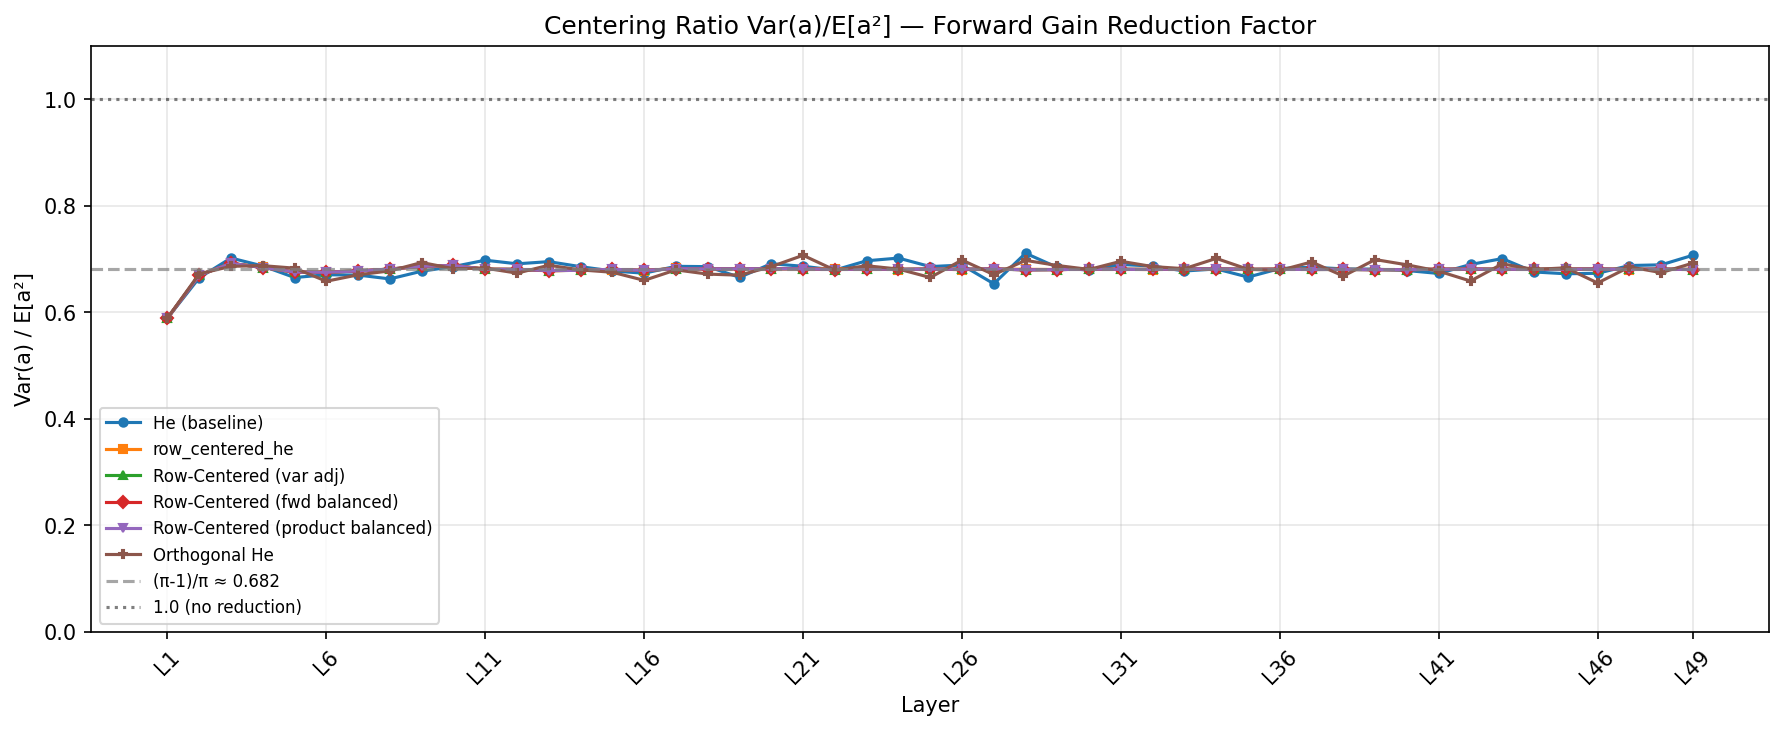
\includegraphics[width=0.85\textwidth]{figures/centering_ratio.png}
\caption{Empirical centering ratio $\Var(a)/\E[a^2]$ per layer.
  All four initializers converge to $({\pi-1})/{\pi} \approx 0.682$,
  confirming this is a universal property of post-ReLU activations.
  Source: \texttt{notebooks/06\_gradient\_diagnostics.ipynb}, Cell~10.}
\label{fig:centering_ratio}
\end{figure}

\subsection{DC/AC decomposition}
\label{sec:dc_ac}

A post-ReLU activation vector at layer~$l$ has $d$ components (one per
neuron in that layer):
$\bm{a}^{(l)} = (a_1, \dots, a_d) \in \R^d$.
Each component can be decomposed into its mean plus deviation:
\begin{equation}\label{eq:dc_ac}
  a_j = \underbrace{\bar{a}}_{\text{DC (mean)}}
      + \underbrace{(a_j - \bar{a})}_{\text{AC (deviation)}},
  \qquad \bar{a} = \frac{1}{d}\sum_{j=1}^{d} a_j.
\end{equation}

\textbf{What is ``energy''?}
In signal processing, the \emph{energy} of a signal
$\{a_1, \dots, a_d\}$ is $\sum_j a_j^2$.  The average per-element
energy is $\frac{1}{d}\sum_j a_j^2 \approx \E[a^2]$
(by the law of large numbers when $d$ is large).
This second moment measures how large the activations are on average,
regardless of sign.

\textbf{Why $\E[a^2]$ splits into DC + AC.}
From the standard variance decomposition:
\[
  \E[a^2] = \underbrace{(\E[a])^2}_{\text{DC energy}}
           + \underbrace{\Var(a)}_{\text{AC energy}}.
\]
\begin{itemize}
  \item \textbf{DC energy} $(\E[a])^2 = \sigma^2/(2\pi)$:
        This is the energy of the \emph{constant} (mean) component.
        By analogy with electrical signals, this is the ``DC'' (direct
        current) component --- a constant offset that is the
        \emph{same for all inputs}.  Whether we feed in a shoe, a shirt,
        or a bag, the mean activation $\E[a] = \sigma/\sqrt{2\pi}$
        is always the same.  It carries \textbf{zero information}
        about the class.

  \item \textbf{AC energy} $\Var(a) = \sigma^2(\pi-1)/(2\pi)$:
        This is the energy of the \emph{fluctuating} component ---
        the ``AC'' (alternating current) part that varies from input
        to input.  The deviations $(a_j - \bar{a})$ are different for
        different inputs, so they preserve the structure of the data.
        This is the \textbf{informative} part.
\end{itemize}

\noindent
The fraction of energy that is informative:
$\text{AC}/\text{total} = (\pi-1)/\pi \approx 68.2\%$.
The remaining $1/\pi \approx 31.8\%$ is uninformative DC ---
a constant offset present in every activation vector,
useless for distinguishing classes.

\subsection{Why row-centered weights are blind to DC}

\begin{proposition}[DC blindness]
\label{prop:dc_blind}
If $\sum_j W_{ij} = 0$ (row centering), then
\[
  z_i = \sum_j W_{ij}\, a_j = \sum_j W_{ij}\,(a_j - \bar{a}).
\]
The neuron's output depends only on the AC component of its input.
\end{proposition}

\begin{proof}
We split each activation into its mean plus deviation.
When row-centered weights ($\sum_j W_{ij} = 0$) multiply the mean
part, it vanishes:
\[
  \sum_j W_{ij}\, a_j
  = \sum_j W_{ij}\,\bar{a} + \sum_j W_{ij}\,(a_j - \bar{a})
  = \bar{a}\underbrace{\sum_j W_{ij}}_{=\,0}
    + \sum_j W_{ij}\,(a_j - \bar{a})
  = \sum_j W_{ij}\,(a_j - \bar{a}).
  \qedhere
\]
\end{proof}

\noindent
\textbf{Consequence for signal propagation.}
When standard He weights compute $z_i = \sum_j W_{ij}\, a_j$, the
weights see the full activation vector including its positive mean.
The variance of the pre-activation is:
\[
  \Var(z_i) = d \cdot \Var(W) \cdot \E[a^2]
  \quad\text{--- uses the \emph{full} second moment $\E[a^2]$.}
\]

When row-centered weights compute the same sum, the DC part vanishes
(Proposition~\ref{prop:dc_blind}), so effectively
$z_i = \sum_j W_{ij}(a_j - \bar{a})$.  The variance becomes:
\[
  \Var(z_i) = d \cdot \Var(W) \cdot \Var(a)
  = d \cdot \Var(W) \cdot \frac{\pi-1}{\pi}\,\E[a^2].
\]

The factor $(\pi-1)/\pi \approx 0.682$ means row-centered weights
produce pre-activations with only $68.2\%$ of the energy that He
weights produce.  This is the energy deficit that compounds across
layers.

% ──────────────────────────────────────────────────────────────────
\section{Forward Gain Derivation}
\label{sec:fwd_gain_derivation}

\subsection{Standard He: forward gain $= 1$}

For a He-initialized layer (no centering), the expected output energy
is:
\begin{equation}\label{eq:he_energy}
  \E[(a^{(l)})^2]
  = \underbrace{\Var(W) \cdot d}_{= (2/d)\cdot d = 2}
  \cdot \underbrace{\frac{1}{2}}_{\text{ReLU survival}}
  \cdot \E[(a^{(l-1)})^2]
  = \E[(a^{(l-1)})^2].
\end{equation}
The forward gain is $g_{\mathrm{fwd}}^{\mathrm{He}} = \sqrt{\E[(a^{(l)})^2] / \E[(a^{(l-1)})^2]} = 1$.

\subsection{Row-centered: forward gain $= \sqrt{(\pi-1)/\pi}$}

The key step: in the He derivation~\eqref{eq:he_energy}, the factor
$\E[(a^{(l-1)})^2]$ appears because He weights see the \emph{full}
activation energy.  For row-centered weights, we must replace this
with $\Var(a^{(l-1)})$ (because of DC blindness,
Proposition~\ref{prop:dc_blind}).  Since
$\Var(a) = \frac{\pi-1}{\pi}\,\E[a^2]$
(Proposition~\ref{prop:centering_ratio}), we get the extra factor
$(\pi-1)/\pi$.

For a row-centered layer with variance-adjusted weights
($\Var(W_{ij}) = 2/d$):

\begin{equation}\label{eq:rc_energy}
  \E[(a^{(l)})^2]
  = \underbrace{\Var(W) \cdot d \cdot \frac{1}{2}}_{= 1}
  \cdot \underbrace{\Var(a^{(l-1)})}_{\text{only AC visible}}
  = \Var(a^{(l-1)})
  = \frac{\pi-1}{\pi}\,\E[(a^{(l-1)})^2].
\end{equation}

This gives a multiplicative recurrence in the energy:
\[
  \E[(a^{(l)})^2] = \frac{\pi-1}{\pi}\,\E[(a^{(l-1)})^2].
\]
At every layer, row-centered weights produce activations whose energy
is $(\pi-1)/\pi \approx 0.682$ times the energy of the previous
layer's activations.  The signal shrinks at every layer.

The forward gain is the ratio of \textbf{amplitudes} (RMS), not energies:
\begin{equation}\label{eq:rc_fwd_gain}
  \boxed{
  g_{\mathrm{fwd}}^{\mathrm{RC}}
  = \sqrt{\frac{\E[(a^{(l)})^2]}{\E[(a^{(l-1)})^2]}}
  = \sqrt{\frac{\pi-1}{\pi}}
  \approx 0.826.
  }
\end{equation}

\begin{remark}[Amplitude vs.\ energy ratio]
\label{rem:amplitude}
The forward gain is defined as
$g_{\mathrm{fwd}} = \rms(A^{(l)}) / \rms(A^{(l-1)})$,
which is a ratio of \emph{amplitudes} (RMS values).
Since $\rms^2 \propto \E[a^2]$ (energy), we have
\[
  g_{\mathrm{fwd}}^2
  = \frac{\E[(a^{(l)})^2]}{\E[(a^{(l-1)})^2]}
  = \frac{\pi-1}{\pi}
  \approx 0.682.
\]
Taking the square root:
$g_{\mathrm{fwd}} = \sqrt{0.682} \approx 0.826$.

\emph{Analogy:} if you halve the power of a light bulb
(energy ratio~$= 1/2$), the brightness (amplitude) drops by
$\sqrt{1/2} \approx 0.707$, not by~$1/2$.
Similarly, an energy ratio of $0.682$ corresponds to an amplitude
ratio of $\sqrt{0.682} = 0.826$.
\end{remark}

\begin{figure}[h]
\centering
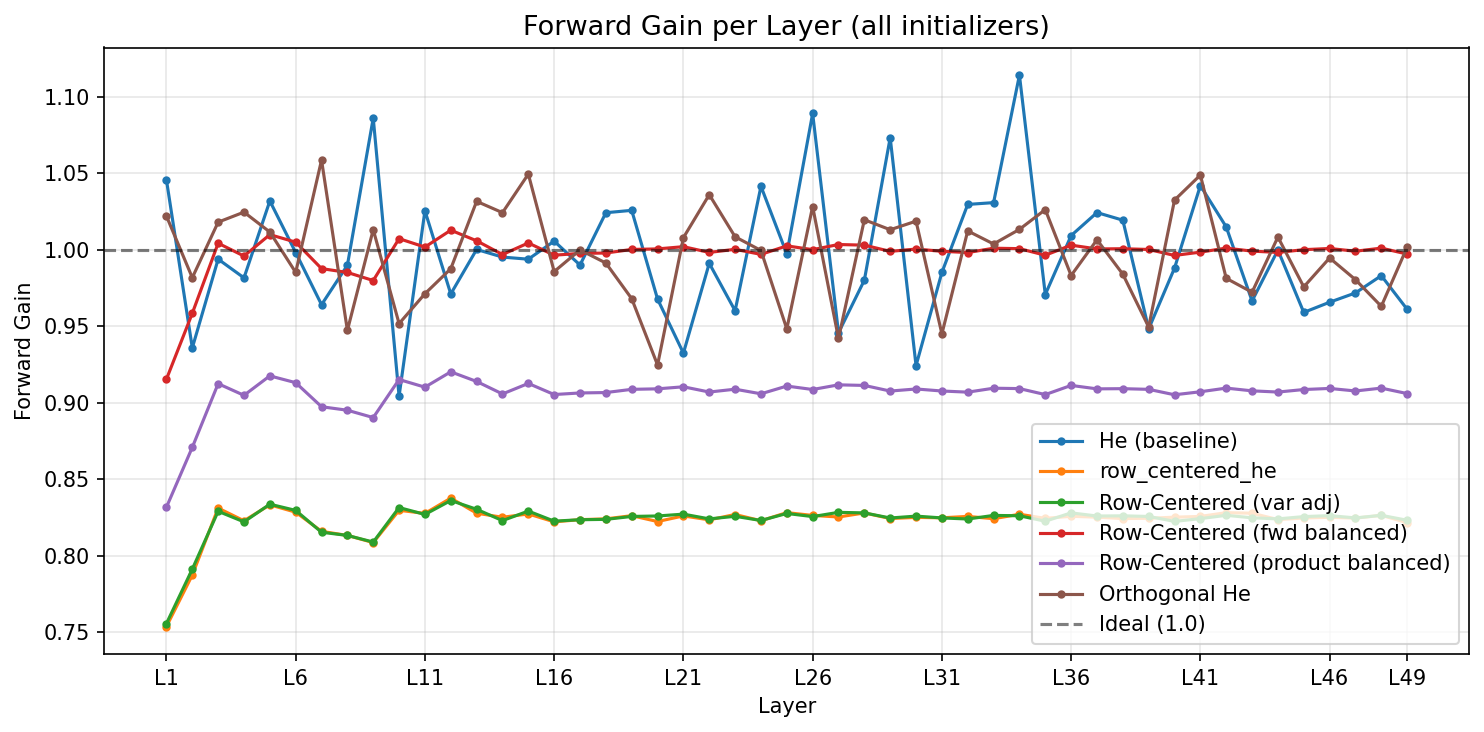
\includegraphics[width=0.85\textwidth]{figures/forward_gain_per_layer.png}
\caption{Forward gain per layer for four initializers (50 hidden layers,
  width~784, Fashion-MNIST).  He and RC~fwd-balanced achieve gain $\approx 1.0$;
  RC~var-adj and \texttt{row\_centered\_he} are locked at $\approx 0.826$.
  Source: \texttt{notebooks/06\_gradient\_diagnostics.ipynb}, Cell~8.}
\label{fig:forward_gain}
\end{figure}

\begin{figure}[h]
\centering
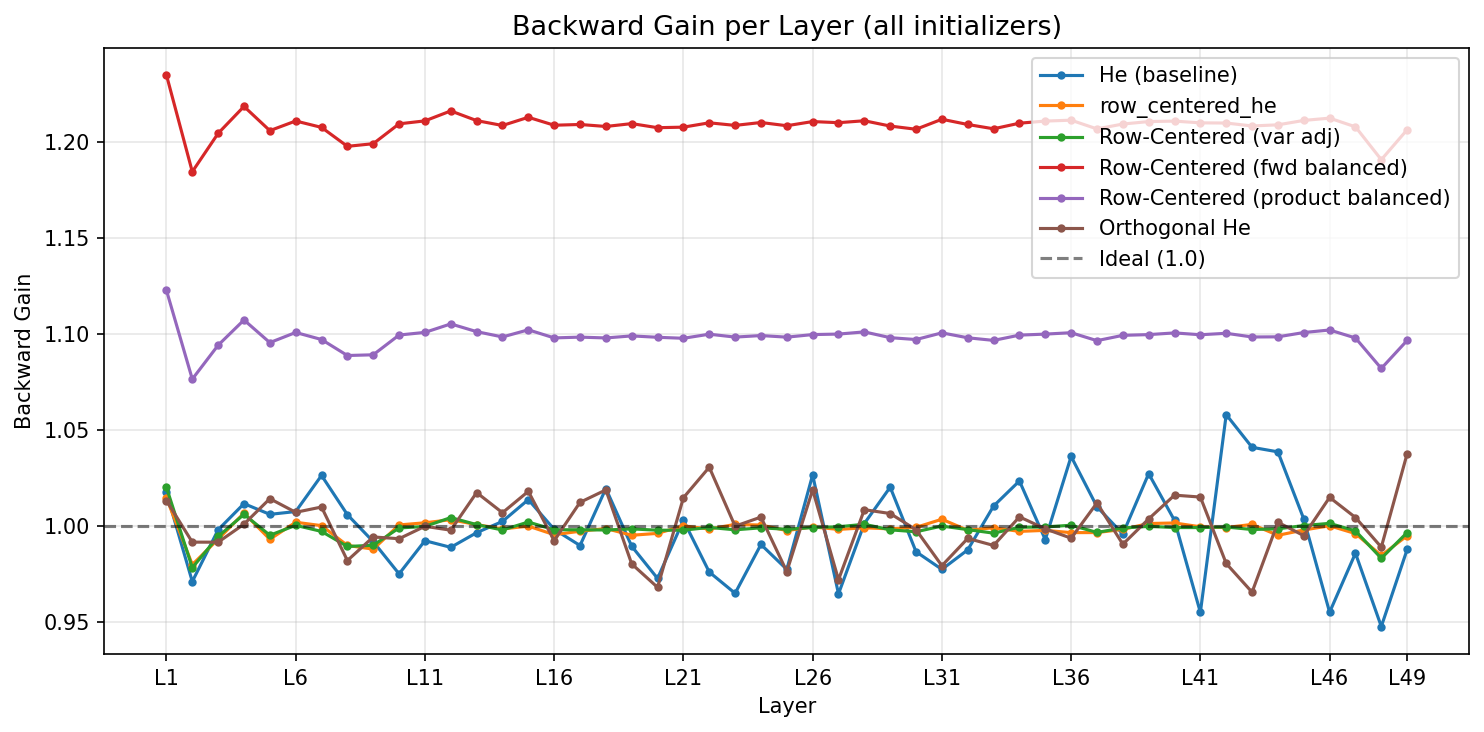
\includegraphics[width=0.85\textwidth]{figures/backward_gain_per_layer.png}
\caption{Backward gain per layer.  He, RC~var-adj, and
  \texttt{row\_centered\_he} all have gain $\approx 1.0$.
  RC~fwd-balanced has gain $\approx 1.21$ --- error signals
  explode at $1.21^{50} \approx 1.3 \times 10^4$.
  Source: \texttt{notebooks/06\_gradient\_diagnostics.ipynb}, Cell~8.}
\label{fig:backward_gain}
\end{figure}

\subsection{Compounding over depth}

Over $L$ layers:
\begin{equation}\label{eq:compounding}
  \rms(a^{(L)}) = \left(\frac{\pi-1}{\pi}\right)^{L/2} \rms(a^{(0)})
  \approx 0.826^L \cdot \rms(a^{(0)}).
\end{equation}

\begin{center}
\begin{tabular}{cc}
\toprule
Depth $L$ & Forward attenuation $0.826^L$ \\
\midrule
10 & $0.147$ \quad ($6.8\times$ decay) \\
20 & $0.022$ \quad ($46\times$ decay) \\
50 & $7.1 \times 10^{-5}$ \quad ($14{,}000\times$ decay) \\
\bottomrule
\end{tabular}
\end{center}

By layer~50, the activations are $14{,}000$ times smaller than the
input.  From~\eqref{eq:grad_magnitude}, the gradient at layer~$l$ is
proportional to $\|\bm{a}^{(l-1)}\|$, so later layers receive
vanishingly small gradients.

% ──────────────────────────────────────────────────────────────────
\section{Why the Backward Gain Is Unaffected}
\label{sec:bwd_gain}

The backward pass propagates the error signal via:
\begin{equation}\label{eq:backward}
  \bm{\delta}^{(l)}
  = \bigl(W^{(l+1)}\bigr)^\top \bm{\delta}^{(l+1)}
    \odot \sigma'(\bm{z}^{(l)}),
\end{equation}
where $\sigma'(\bm{z}^{(l)}) = \mathbf{1}[\bm{z}^{(l)} > 0]$ is the
ReLU derivative (binary mask).

If $W$ is row-centered ($\sum_j W_{ij} = 0$), then $W^\top$ is
\emph{column-centered} ($\sum_i W_{ij} = 0$ for each column~$j$).
Applying $W^\top$ to $\bm{\delta}^{(l+1)}$ gives:
\[
  (W^\top \bm{\delta})_j = \sum_i W_{ij}\,\delta_i.
\]
The centering of columns means this is blind to the mean of
$\bm{\delta}^{(l+1)}$.  However, unlike post-ReLU activations, the
error signal $\bm{\delta}$ has \textbf{near-zero mean} (it contains
both positive and negative values).  Therefore:
\[
  \frac{\Var(\delta)}{\E[\delta^2]}
  = 1 - \frac{(\E[\delta])^2}{\E[\delta^2]}
  \approx 1,
\]
and the column centering of $W^\top$ has negligible effect on the
backward signal energy.

\begin{proposition}[Forward-backward gain ratio]
\label{prop:fb_ratio}
For row-centered initialization with any weight variance:
\begin{equation}\label{eq:fb_ratio}
  \frac{g_{\mathrm{fwd}}}{g_{\mathrm{bwd}}}
  = \sqrt{\frac{\pi-1}{\pi}}
  \approx 0.827.
\end{equation}
This ratio is \textbf{independent of the weight variance}.
\end{proposition}

This is the fundamental coupling: the forward and backward gains
are locked in a fixed ratio.  No scalar variance adjustment can make
both equal to~1 simultaneously.

% ──────────────────────────────────────────────────────────────────
\section{Empirical Confirmation: Variance Sweep}
\label{sec:var_sweep}

We sweep the variance factor for row-centered initialization from
$1.5/d$ to $3.0/d$:

\begin{center}
\begin{tabular}{cccc}
\toprule
Variance factor & Median fwd gain & Median bwd gain & Ratio F/B \\
\midrule
$1.5/d$ & 0.715 & 0.865 & \textbf{0.827} \\
$2.0/d$ (He) & 0.826 & 0.999 & \textbf{0.827} \\
$2.5/d$ & 0.923 & 1.116 & \textbf{0.827} \\
$3.0/d$ & 1.011 & 1.223 & \textbf{0.827} \\
\bottomrule
\end{tabular}
\end{center}

The ratio $g_{\mathrm{fwd}}/g_{\mathrm{bwd}} = 0.827$ is constant
across all variance factors, confirming
Proposition~\ref{prop:fb_ratio}.

\textbf{Interpretation:}
\begin{itemize}
  \item At $\Var = 2.0/d$: backward gain $= 1.0$ (healthy), but
        forward gain $= 0.826$ (activations vanish).
  \item At $\Var \approx 2.93/d$: forward gain $= 1.0$ (healthy), but
        backward gain $= 1.21$ (error signals explode:
        $1.21^{50} \approx 1.3 \times 10^4$).
  \item No variance gives both $= 1$.
\end{itemize}

\section{The Coupling Formula}
\label{sec:fwd_bwd_coupling}

Writing the forward gain as $g_{\mathrm{fwd}} = r \cdot s$ where
$r = \sqrt{(\pi-1)/\pi} \approx 0.826$ is the structural centering
factor and $s$ depends on the weight variance, and the backward gain as
$g_{\mathrm{bwd}} = s$:

\begin{equation}\label{eq:coupling}
  \frac{g_{\mathrm{fwd}}}{g_{\mathrm{bwd}}} = r \approx 0.826
  \quad\text{always.}
\end{equation}

\begin{itemize}
  \item $s = 1$ (He variance, \texttt{var\_adj}):
        $g_{\mathrm{fwd}} = 0.826$, $g_{\mathrm{bwd}} = 1.0$
        $\Rightarrow$ activations vanish.
  \item $s = 1/r \approx 1.21$ (\texttt{fwd\_balanced}):
        $g_{\mathrm{fwd}} = 1.0$, $g_{\mathrm{bwd}} = 1.21$
        $\Rightarrow$ error signals explode.
  \item Any $s$ in between: both are off from~1.
\end{itemize}

\textbf{This is why geometry (requiring row centering) and gradient
stability (requiring gain $\approx 1$) conflict.}

% ──────────────────────────────────────────────────────────────────
\section{Single vs.\ Multi-Sample: The Trap Is Structural}
\label{sec:single_multi}

To verify that the gradient non-uniformity is not a statistical
artifact of batch aggregation, we compare gradient profiles using
$n = 1$ vs.\ $n = 2000$ samples.

\begin{center}
\begin{tabular}{lcc}
\toprule
Initializer & Log-scale correlation & Interpretation \\
\midrule
He & 0.86 & Noisier (no centering stabilization) \\
RC var-adj & 0.98 & Same pattern \\
RC fwd-balanced & 0.98 & Same pattern \\
\bottomrule
\end{tabular}
\end{center}

The row-centered variants show correlation $> 0.97$ between single-sample
and batch gradient profiles.  The gradient decay pattern is identical
whether we use one data point or two thousand.

\textbf{Conclusion:} The gradient non-uniformity is \textbf{structural}
--- it comes from the weight matrices and the ReLU activation, not from
data aggregation.

% ──────────────────────────────────────────────────────────────────
\section{ReLU Survival Is Not the Issue}
\label{sec:relu_survival}

All three initializers show ReLU survival rates of approximately
$50\% \pm 2\%$ across all layers:

\begin{itemize}
  \item He: $50\% \pm 1.7\%$ (higher noise)
  \item RC var-adj: $50\% \pm 0.4\%$ (tighter due to centering)
  \item RC fwd-balanced: $50\% \pm 0.4\%$
\end{itemize}

Row centering does \textbf{not} kill more neurons than standard He.
The gradient trap is not about dead neurons --- it is about the
\emph{positive mean} of surviving activations (the DC component that
row-centered weights cannot see).

% ══════════════════════════════════════════════════════════════════
\chapter{Attempting to Fix the Trap}
\label{ch:fixing_trap}
% ══════════════════════════════════════════════════════════════════

Chapter~\ref{ch:gradient_trap} established that row centering creates a
locked forward/backward gain ratio of $\sqrt{(\pi-1)/\pi} \approx 0.827$.
This chapter explores two strategies to mitigate the resulting gradient
non-uniformity.

% ──────────────────────────────────────────────────────────────────
\section{Partial Centering (Alpha Sweep)}
\label{sec:alpha_sweep}

\subsection{Definition}

For $\alpha \in [0,1]$, define partial centering:
\begin{equation}\label{eq:partial_centering}
  W_{ij} = W_{ij}^{(\mathrm{He})}
           - \alpha \cdot \bar{w}_i,
  \qquad
  \bar{w}_i = \frac{1}{d}\sum_k W_{ik}^{(\mathrm{He})},
\end{equation}
followed by rescaling each row to restore He variance.
At $\alpha = 0$ this is pure He; at $\alpha = 1$ this is full row
centering.

\subsection{Effect on forward gain}

Partial centering with parameter $\alpha$ suppresses a fraction of the
DC component.  The effective input energy seen by the neuron is
approximately:
\begin{equation}
  E_{\mathrm{eff}} \approx \E[a^2] - \alpha^2 \cdot (\E[a])^2
  = \E[a^2]\left(1 - \frac{\alpha^2}{\pi}\right),
\end{equation}
giving forward gain approximately:
\begin{equation}\label{eq:partial_fwd}
  g_{\mathrm{fwd}}(\alpha) \approx \sqrt{1 - \frac{\alpha^2}{\pi}}
  \approx 1 - \frac{\alpha^2}{2\pi}.
\end{equation}
A simpler linear approximation from the data:
$g_{\mathrm{fwd}}(\alpha) \approx 1 - 0.174\,\alpha$.

\subsection{Empirical results}

\textbf{Setup:} 50 hidden layers, width 784, Fashion-MNIST.
PCA geometry metric (used before the k-NN transition; see
Chapter~\ref{ch:geometry} for why this is misleading).

\begin{center}
\begin{tabular}{ccccc}
\toprule
$\alpha$ & Med fwd gain & Med bwd gain & Grad spread & Geometry (PCA) \\
\midrule
0.0 & 0.996 & 0.997 & $6.6\times$ & 0.955 \\
0.2 & 0.937 & 0.996 & $2.4\times$ & 0.905 \\
0.4 & 0.887 & 0.999 & $36.8\times$ & 0.835 \\
0.6 & 0.853 & 0.998 & $294.7\times$ & 0.822 \\
0.8 & 0.832 & 0.999 & $1{,}219\times$ & 0.808 \\
1.0 & 0.826 & 0.999 & $1{,}908\times$ & 0.818 \\
\bottomrule
\end{tabular}
\end{center}

Key observations:
\begin{enumerate}
  \item \textbf{Backward gain $\approx 1.0$ for all $\alpha$:}
        The backward pass is robust to partial centering because the
        transposed weights interact with error signals that have
        near-zero mean.
  \item \textbf{Gradient spread grows exponentially with $\alpha$:}
        Even $\alpha = 0.5$ gives $g_{\mathrm{fwd}} \approx 0.913$,
        which over 50 layers compounds to $0.913^{50} \approx 0.010$
        --- three orders of magnitude decay.
  \item \textbf{No $\alpha$ gives both good gradients and good geometry:}
        $\alpha = 0.2$ minimizes gradient spread ($2.4\times$) but has
        poor geometry.  $\alpha \geq 0.6$ gives good geometry but
        gradient spreads $> 300\times$.
\end{enumerate}

\begin{figure}[h]
\centering
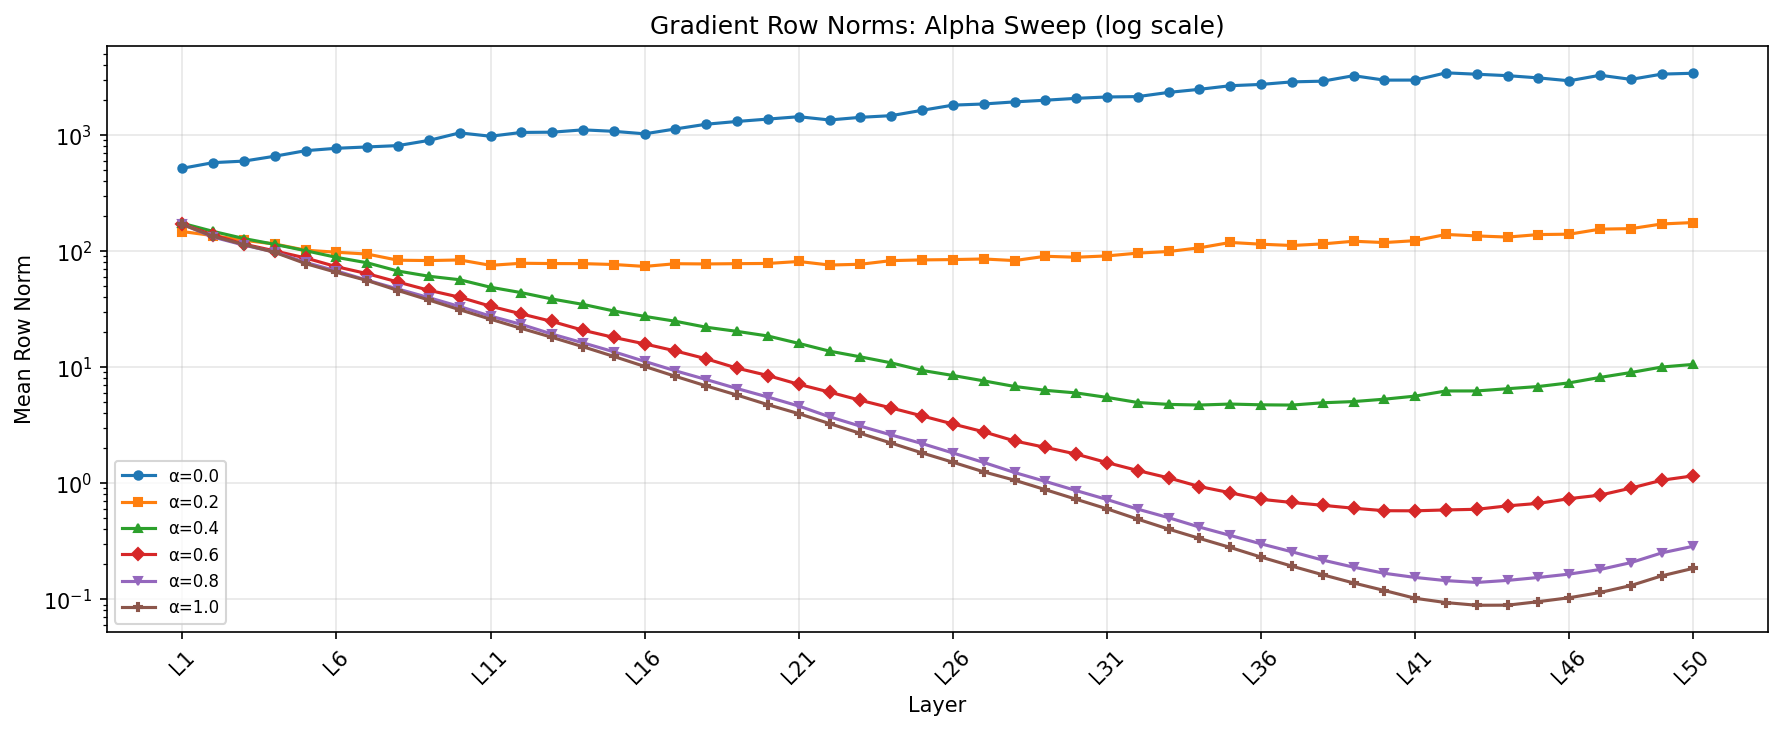
\includegraphics[width=0.85\textwidth]{figures/gradient_norms_alpha_sweep.png}
\caption{Gradient row norms (log scale) across 50 layers for partial centering
  with $\alpha \in \{0, 0.2, 0.4, 0.6, 0.8, 1.0\}$.
  At $\alpha = 0$ (He), gradients are nearly flat.
  At $\alpha = 1$ (full centering), gradients span $\sim\!4$ orders of magnitude.
  Source: \texttt{notebooks/06\_gradient\_diagnostics.ipynb}, Cell~20.}
\label{fig:gradient_norms_alpha}
\end{figure}

\subsection{Conclusion}

Partial centering defines a \textbf{Pareto frontier} between geometry
and gradient uniformity.  It allows choosing \emph{where} on the
trade-off to sit, but cannot escape it.  Any $\alpha$ large enough to
meaningfully suppress DC drift creates enough forward signal loss to
produce non-uniform gradients.

% ──────────────────────────────────────────────────────────────────
\section{Layer-Balanced Initialization (Eta Sweep)}
\label{sec:eta_sweep}

\subsection{Motivation}

The partial centering approach tried to reduce the centering
parameter.  The layer-balanced approach takes a fundamentally different
strategy: \textbf{keep full row centering ($\alpha = 1$) for best
geometry, but use different weight variances at each layer to equalize
gradients despite the forward decay.}

\subsection{Mathematical derivation}

Let each layer $l \in \{1,\dots,L\}$ have weight standard deviation
$s_l$.  From the backpropagation equations:

\textbf{Forward chain} (activation magnitude at layer $l-1$):
\begin{equation}\label{eq:fwd_chain}
  \|\bm{a}^{(l-1)}\| \propto \prod_{k=1}^{l-1} (r \cdot s_k),
\end{equation}
where $r = \sqrt{(\pi-1)/\pi} \approx 0.826$ is the structural
centering loss per layer, and $r \cdot s_k$ is the forward amplitude
gain at layer~$k$.

\textbf{Backward chain} (error signal at layer $l$):
\begin{equation}\label{eq:bwd_chain}
  \|\bm{\delta}^{(l)}\| \propto \prod_{k=l+1}^{L} s_k.
\end{equation}
The backward gain at layer~$k$ is approximately $s_k$ (Section~\ref{sec:bwd_gain}).

\textbf{Gradient at layer $l$} (from BP4, equation~\eqref{eq:bp4}):
\begin{equation}\label{eq:grad_layer}
  \left\|\frac{\partial \mathcal{C}}{\partial W^{(l)}}\right\|
  \propto \|\bm{a}^{(l-1)}\| \cdot \|\bm{\delta}^{(l)}\|
  \propto \prod_{k=1}^{l-1}(r \cdot s_k) \cdot \prod_{k=l+1}^{L} s_k
  = r^{l-1} \cdot \frac{\prod_{k=1}^{L} s_k}{s_l}.
\end{equation}

Since $\prod_{k=1}^{L} s_k$ is a constant (independent of $l$),
the gradient depends on $l$ only through:
\begin{equation}\label{eq:grad_prop}
  \left\|\frac{\partial \mathcal{C}}{\partial W^{(l)}}\right\|
  \propto \frac{r^{l-1}}{s_l}.
\end{equation}

\textbf{For uniform gradients}, we need $r^{l-1}/s_l = \text{const}$,
which gives:
\begin{equation}\label{eq:optimal_sl}
  s_l \propto r^{l-1}.
\end{equation}

Early layers ($l$ small) get $s_l$ large (boosted weights);
late layers ($l$ large) get $s_l$ small (reduced weights).

\subsection{Parameterization}

We center the scaling at the middle layer and introduce a strength
parameter $\eta$:
\begin{equation}\label{eq:sl_param}
  s_l = r^{\,\eta \cdot (l - (L+1)/2)},
\end{equation}
so that $s_{(L+1)/2} = 1$ (middle layer unchanged).

\begin{itemize}
  \item $\eta = 0$: $s_l = 1$ for all $l$ (no correction).
  \item $\eta = 1$: full correction ($s_l = r^{l-(L+1)/2}$).
  \item $\eta = 0.5$: half correction.
\end{itemize}

The total weight std at layer $l$ is
$\sigma_l = \sigma_{\mathrm{base}} \cdot s_l$, where
$\sigma_{\mathrm{base}} = \sqrt{2/d} \cdot \sqrt{\pi/(\pi-1)}$
is the forward-balanced base (see the flag in
Section~\ref{sec:layer_balanced}).

\subsection{Results}

\textbf{Setup:} 20 hidden layers, width 784, Fashion-MNIST.

\begin{center}
\begin{tabular}{ccccc}
\toprule
Config & Grad ratio & Grad CV & Med fwd gain & Med bwd gain \\
\midrule
He (baseline) & $1.93\times$ & 0.182 & 0.979 & 1.022 \\
$\eta = 0.00$ & $11.41\times$ & 0.926 & 0.999 & 1.213 \\
$\eta = 0.25$ & $6.52\times$ & 0.603 & 1.045 & 1.212 \\
$\bm{\eta = 0.50}$ & $\bm{4.32\times}$ & \textbf{0.521} & 1.096 & 1.212 \\
$\eta = 0.75$ & $6.67\times$ & 0.764 & 1.150 & 1.212 \\
$\eta = 1.00$ & $12.93\times$ & 1.075 & 1.206 & 1.212 \\
\bottomrule
\end{tabular}
\end{center}

\begin{flagbox}
At $\eta = 0$, the median forward gain is $0.999$ and the backward
gain is $1.213$.  This means $\eta = 0$ corresponds to the
\textbf{forward-balanced} base (Section~\ref{sec:rc_fwd_balanced}),
\emph{not} the variance-adjusted base (which would give forward
gain $\approx 0.826$ and backward gain $\approx 1.0$).
\end{flagbox}

\subsection{Analysis}

\begin{enumerate}
  \item \textbf{$\eta = 0.5$ is the sweet spot:}
        Gradient ratio improves from $11.41\times$ to $4.32\times$
        ($\sim 2.6\times$ improvement), CV from 0.926 to 0.521.
        Still worse than He's $1.93\times$.

  \item \textbf{$\eta = 1.0$ is worse than $\eta = 0$:}
        Gradient ratio $12.93\times$ vs.\ $11.41\times$.
        The full correction \textbf{overshoots}.

  \item \textbf{Backward gain is $1.21$ for ALL $\eta$:}
        The backward gain depends on the average weight scale
        (the forward-balanced base), not on how variance is
        distributed across layers.
        Over 20 layers: $1.21^{20} \approx 55\times$ backward
        amplification.
\end{enumerate}

\begin{figure}[h]
\centering
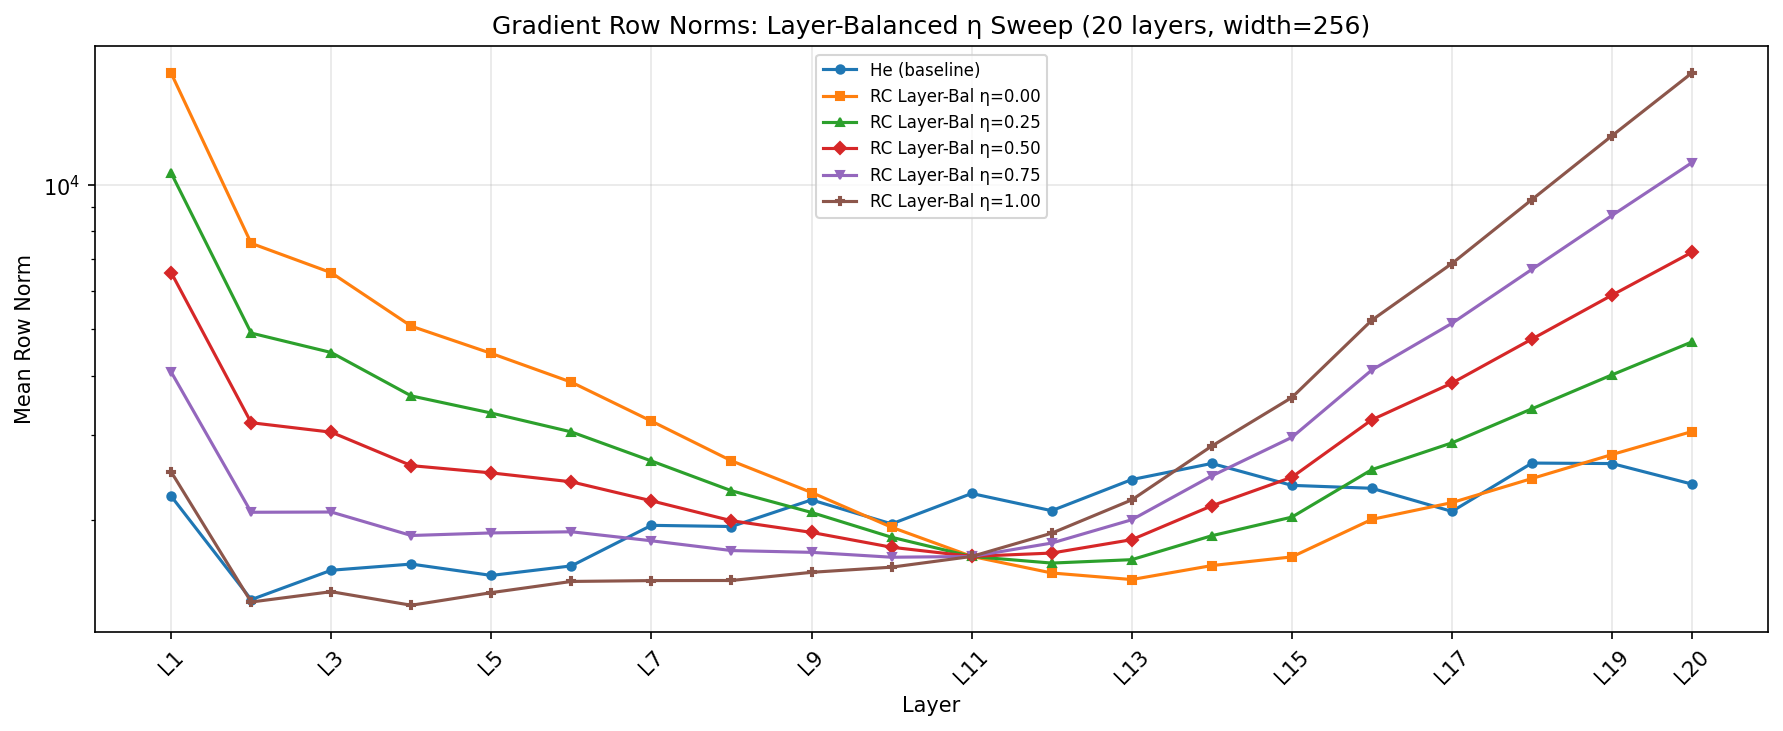
\includegraphics[width=0.85\textwidth]{figures/gradient_norms_eta_sweep.png}
\caption{Gradient row norms (log scale) for layer-balanced initialization
  with $\eta \in \{0, 0.25, 0.5, 0.75, 1.0\}$ and He baseline.
  $\eta = 0.5$ achieves the flattest profile among row-centered variants.
  Source: \texttt{notebooks/06\_gradient\_diagnostics.ipynb}, Cell~23.}
\label{fig:gradient_norms_eta}
\end{figure}

\subsection{Why $\eta = 1$ overshoots}

At $\eta = 1$, the per-layer scaling
$s_l = r^{l - (L+1)/2}$ fully compensates forward decay.
But it also makes the backward gain \textbf{non-uniform}:

\begin{itemize}
  \item Early layers: $s_l > 1$ (boosted weights) $\Rightarrow$
        backward gain $= 1.21 \times s_l \gg 1$
        (up to ${\sim}7$ in the empirical plot).
  \item Late layers: $s_l < 1$ (reduced weights) $\Rightarrow$
        backward gain $= 1.21 \times s_l < 1$.
\end{itemize}

The layer-dependent $s_l$ that fixes the forward chain
\textbf{destabilizes the backward chain}.
At $\eta = 0.5$, the partial compensation balances forward improvement
against backward destabilization.

\subsection{Comparison to partial centering}

\begin{center}
\begin{tabular}{lccc}
\toprule
Approach & Gradient spread & Geometry & Mechanism \\
\midrule
Partial centering ($\alpha = 0.25$) & $6.6\times$ & Poor & Reduce centering \\
Layer-balanced ($\eta = 0.5$) & $4.32\times$ & Best (full RC) & Redistribute variance \\
\bottomrule
\end{tabular}
\end{center}

The layer-balanced approach is \textbf{strictly better on the Pareto
frontier}: it achieves lower gradient spread ($4.32\times$ vs.\
$6.6\times$) while maintaining full row-centered geometry.

\subsection{Fundamental limitation}

The backward gain of $1.21$ (from the forward-balanced base) limits
how much the layer-balanced approach can improve.
The $\eta$ parameter redistributes gradient non-uniformity between
forward and backward chains but cannot eliminate it.
The optimal $\eta \approx 0.5$ represents the point where forward
compensation and backward destabilization are balanced.

% ══════════════════════════════════════════════════════════════════
\chapter{Geometry Revisited: The PCA Metric Was Wrong}
\label{ch:geometry}
% ══════════════════════════════════════════════════════════════════

\noindent
\textbf{Experimental setup.}
Fashion-MNIST (2000 samples), depths $L \in \{5, 10, 15, 20\}$,
width~784 (square projections).  Five initializers compared using the
three geometry metrics from Section~\ref{sec:geometry_metrics}.

% ──────────────────────────────────────────────────────────────────
\section{$k$-NN Results Overturn the Narrative}

\begin{table}[h]
\centering
\begin{tabular}{lcccc}
\toprule
Initializer & 5\,L & 10\,L & 15\,L & 20\,L \\
\midrule
\texttt{he}                          & 0.736 & 0.710 & 0.673 & \textbf{0.639} \\
\texttt{orthogonal\_he}              & \textbf{0.755} & \textbf{0.724} & \textbf{0.696} & \textbf{0.662} \\
\texttt{orthogonal\_tuned}           & 0.755 & 0.724 & 0.696 & 0.662 \\
\texttt{row\_centered\_he\_var\_adj} & 0.717 & 0.482 & 0.186 & 0.110 \\
\texttt{kernel\_preserving}          & 0.737 & 0.628 & 0.540 & 0.100 \\
\bottomrule
\end{tabular}
\caption{$k$-NN accuracy ($k=5$) vs.\ depth.
  Chance level $= 0.10$ (10 classes).}
\label{tab:knn}
\end{table}

\textbf{The key finding:}
Row-centered var-adj drops from 0.717 (5\,L) to \textbf{0.110} (20\,L)
--- indistinguishable from \textbf{chance level}.
Meanwhile He degrades gracefully from 0.736 to 0.639, losing only
$\sim$13\% of its class separability over 20 layers.

This directly contradicts the PCA scatter plot evidence from earlier
work, which suggested row centering ``preserves geometry'' better
than~He.

\begin{figure}[h]
\centering
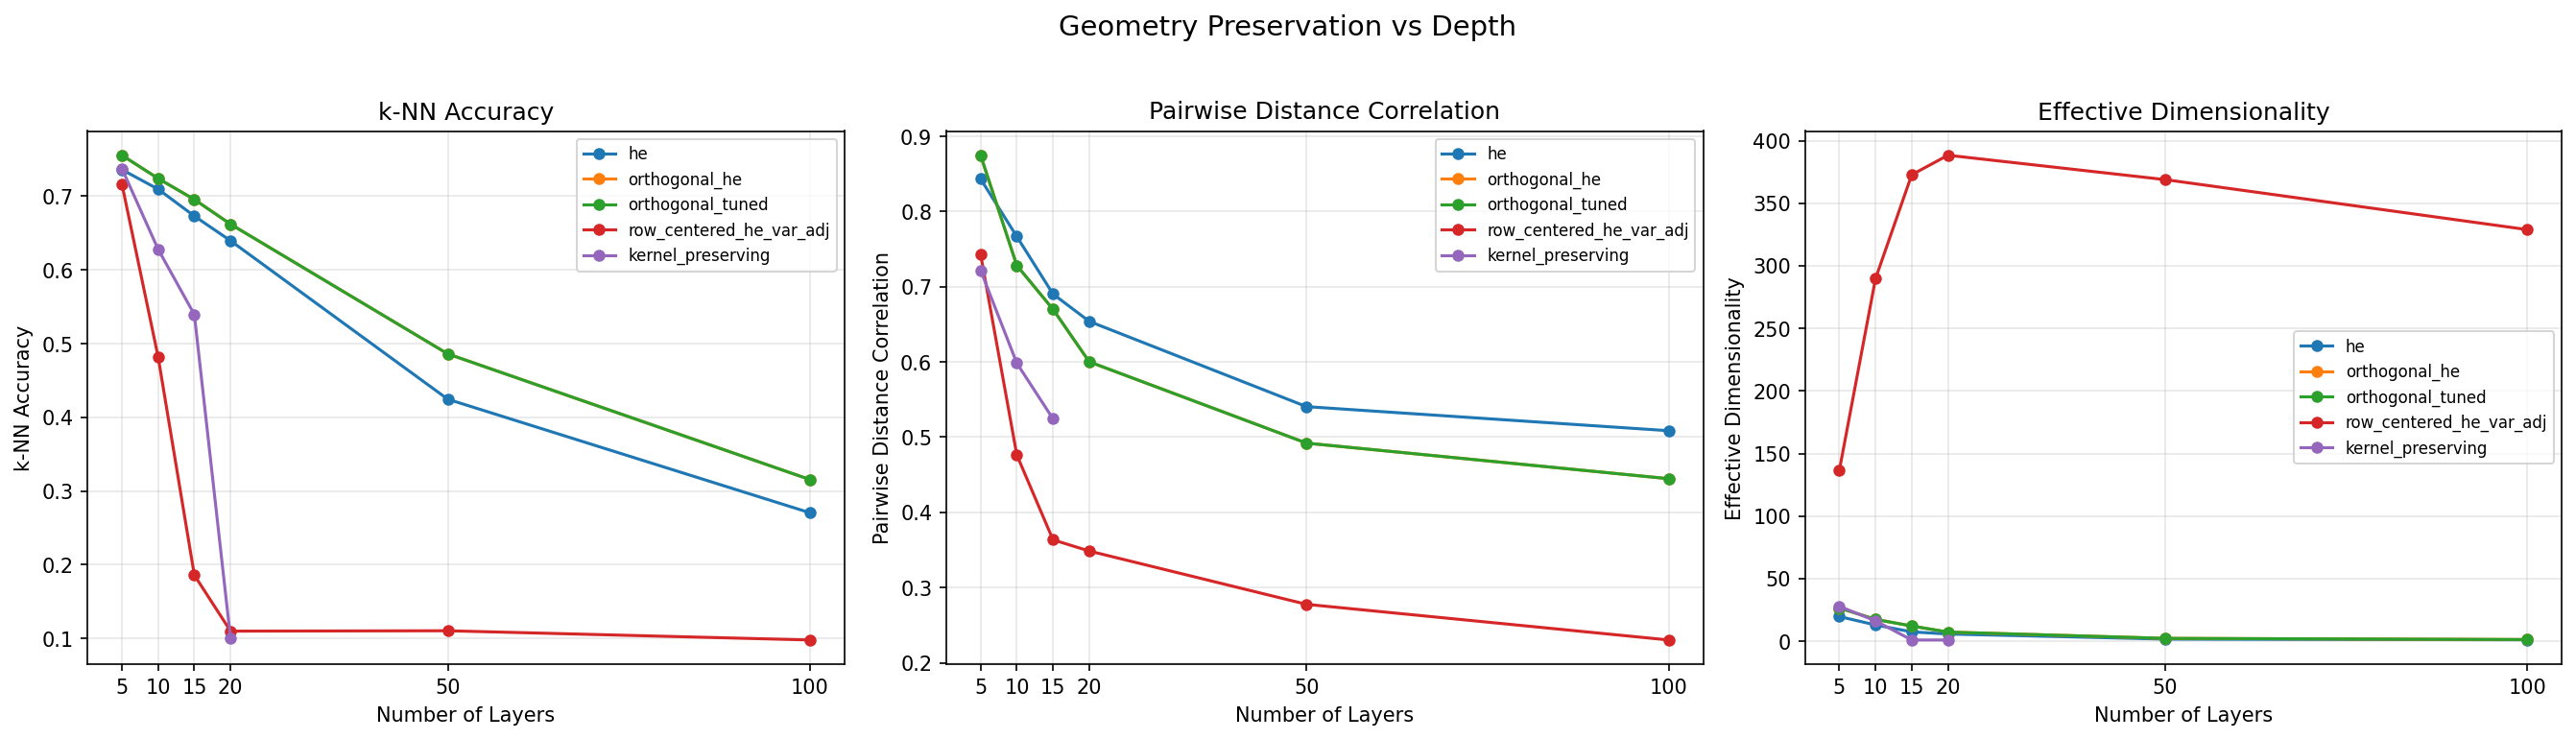
\includegraphics[width=\textwidth]{figures/geometry_vs_depth.png}
\caption{Three geometry metrics vs.\ depth for five initializers.
  \textbf{Left:} $k$-NN accuracy --- row-centered drops to chance (0.10)
  by 20~layers while He stays at 0.64.
  \textbf{Center:} Pairwise distance correlation.
  \textbf{Right:} Effective dimensionality --- row-centered has high
  $d_{\mathrm{eff}}$ (spread-out noise) despite zero class structure.
  Source: \texttt{notebooks/07\_kernel\_geometry\_analysis.ipynb}, Cell~6.}
\label{fig:geometry_vs_depth}
\end{figure}

\begin{table}[h]
\centering
\begin{tabular}{lcccc}
\toprule
Initializer & 5\,L & 10\,L & 15\,L & 20\,L \\
\midrule
\texttt{he}                          & 0.843 & 0.767 & 0.690 & 0.654 \\
\texttt{orthogonal\_he}              & \textbf{0.875} & 0.728 & 0.670 & 0.600 \\
\texttt{row\_centered\_he\_var\_adj} & 0.743 & 0.476 & 0.363 & 0.349 \\
\texttt{kernel\_preserving}          & 0.722 & 0.598 & 0.524 & NaN \\
\bottomrule
\end{tabular}
\caption{Pairwise distance correlation (Spearman) vs.\ depth.}
\label{tab:dist_corr}
\end{table}

\begin{table}[h]
\centering
\begin{tabular}{lcccc}
\toprule
Initializer & 5\,L & 10\,L & 15\,L & 20\,L \\
\midrule
\texttt{he}                          & 19.7 & 13.0 & 7.5 & 5.8 \\
\texttt{orthogonal\_he}              & 26.6 & 17.5 & 12.2 & 7.3 \\
\texttt{row\_centered\_he\_var\_adj} & \textbf{136.2} & \textbf{289.7} & \textbf{372.7} & \textbf{388.3} \\
\texttt{kernel\_preserving}          & 28.0 & 16.3 & 1.0 & 1.0 \\
\bottomrule
\end{tabular}
\caption{Effective dimensionality (eigenvalue entropy) vs.\ depth.}
\label{tab:eff_dim}
\end{table}

% ──────────────────────────────────────────────────────────────────
\section{Why the PCA Metric Was Misleading}
\label{sec:pca_misleading}

The effective dimensionality reveals the mechanism:
\begin{itemize}
  \item \textbf{Row-centered}: $d_{\mathrm{eff}} = 388$ at 20\,L
        (data spread across $\sim$388 dimensions).
  \item \textbf{He}: $d_{\mathrm{eff}} = 5.8$ at 20\,L
        (data compressed into $\sim$6 dimensions).
\end{itemize}

The PCA scatter plots showed row-centered data ``spreading out'' in the
first two principal components --- which \emph{looks like} preserved
structure.  But \textbf{spread $\neq$ structure}:

\begin{enumerate}
  \item The forward signal decays by $0.826^L$ per layer
        (equation~\eqref{eq:compounding}).
  \item By 20 layers: $0.826^{20} \approx 0.022$, so activations are
        $\sim\!46\times$ smaller than the input.
  \item At this scale, the signal is dominated by random fluctuations
        from weight initialization, not input structure.
  \item The data becomes \textbf{uniformly dispersed noise}: high
        dimensional (high $d_{\mathrm{eff}}$) but with
        \emph{no class information} ($k$-NN $=$ chance).
\end{enumerate}

He, by contrast, compresses data into fewer dimensions (low
$d_{\mathrm{eff}}$), but the \textbf{class structure is preserved
within those dimensions}.  The angular contraction from the ReLU kernel
($D(\alpha) > 0$) compresses representations but maintains relative
ordering of inter-class vs.\ intra-class distances.

\begin{remark}[Effective dimensionality is misleading in isolation]
High $d_{\mathrm{eff}}$ combined with low $k$-NN accuracy indicates
uniformly dispersed noise, not good geometry.
Low $d_{\mathrm{eff}}$ combined with high $k$-NN accuracy indicates
efficient compression with preserved class structure.
The $k$-NN accuracy is the correct primary metric.
\end{remark}

% ──────────────────────────────────────────────────────────────────
\section{Orthogonal Initialization Analysis}
\label{sec:orthogonal_analysis}

\subsection{Same expected kernel as He}

\begin{proposition}
For a square orthogonal matrix $W = \sqrt{2}\,Q$ (where $Q$ is from QR
decomposition), the expected kernel per neuron is the same as for
i.i.d.\ Gaussian weights with matching variance.
\end{proposition}

\begin{proof}[Proof sketch]
Each row $\bm{w}_k$ of the orthogonal matrix, viewed in isolation,
is uniformly distributed on the sphere of radius $\sqrt{2}$.
This is the same distribution as a normalized Gaussian vector
$\sqrt{2}\,\bm{g}/\|\bm{g}\|$ where $\bm{g} \sim \mathcal{N}(\bm{0}, I)$.
In the large-$d$ limit, $\|\bm{g}\| \approx \sqrt{d}$ concentrates, so
the marginal distribution of $\bm{w}_k$ approaches
$\mathcal{N}(\bm{0}, (2/d)\,I)$ --- the same as He.

The kernel proof (Theorem~\ref{thm:kernel}) computes
$\E[\relu(\bm{w}_k^\top \bm{x}_i) \cdot \relu(\bm{w}_k^\top \bm{x}_j)]$,
which depends only on the marginal distribution of individual rows.
Since orthogonal rows have the same marginal as Gaussian rows, the
expected kernel per neuron is identical.
\end{proof}

\textbf{What orthogonal changes:} The rows are no longer independent
(they are mutually orthogonal), so the \emph{variance} of the kernel
estimate decreases (better concentration).  The \emph{expectation} is
still $K(\alpha)$ with the same distortion $D(\alpha) > 0$.

\textbf{Prediction confirmed:} Orthogonal shows the same systematic
collapse rate as He, with ${\sim}3.6\%$ improvement from reduced noise
($0.662$ vs.\ $0.639$ at 20\,L).

\subsection{Orthogonal\_he equals orthogonal\_tuned}

With square matrices ($784 \times 784$) and the same seed, QR produces
the same orthogonal matrix $Q$.  The only difference is the gain:
$\sqrt{2}\,Q$ vs.\ $\sqrt{1.65}\,Q$.  Since all three geometry metrics
($k$-NN, Spearman distance correlation, effective dimensionality) are
\textbf{scale-invariant}, the two produce identical results.

% ──────────────────────────────────────────────────────────────────
\section{Kernel-Preserving Failure at Depth}
\label{sec:kp_failure}

\begin{center}
\begin{tabular}{ccccc}
\toprule
Depth & $k$-NN & Dist.\ corr. & $d_{\mathrm{eff}}$ & Status \\
\midrule
5\,L  & 0.737 & 0.722 & 28.0 & Comparable to He \\
10\,L & 0.628 & 0.598 & 16.3 & Degrading \\
15\,L & 0.540 & 0.524 & 1.0  & Numerical collapse \\
20\,L & 0.100 & NaN   & 1.0  & Overflow \\
\bottomrule
\end{tabular}
\end{center}

The kernel-preserving optimizer (Section~\ref{sec:kp_init}) optimizes
each layer independently via 200~Adam steps.  It does not account for
how previous layers have already transformed the data.

\begin{itemize}
  \item At 5\,L: comparable to He ($0.737$ vs.\ $0.736$).
  \item At 15\,L: $d_{\mathrm{eff}} = 1.0$ --- data has collapsed to a
        single direction.
  \item At 20\,L: $k$-NN $= 0.100$ (chance), distance correlation $=$ NaN
        (float64 overflow from accumulated weight inflation of
        ${\sim}15^{20}$).
\end{itemize}

Per-layer optimization is \textbf{non-composable}: each layer is
locally optimal, but the composition of 15+ independently-optimized
layers diverges.

% ──────────────────────────────────────────────────────────────────
\section{Revised Narrative}
\label{sec:revised_narrative}

The previous argument was:
\begin{quote}
\emph{``Row centering preserves geometry but creates a gradient trap.''}
\end{quote}

The corrected argument is:
\begin{quote}
\textbf{Row centering prevents angular collapse but destroys class
structure (via forward signal decay) AND creates a gradient trap.
These are the same phenomenon --- the forward decay kills both.}
\end{quote}

Row centering:
\begin{enumerate}
  \item Does \textbf{NOT} preserve geometry (as measured by class
        separability / $k$-NN accuracy).
  \item \textbf{DOES} prevent angular collapse (data stays spread out
        --- high $d_{\mathrm{eff}}$).
  \item But ``staying spread out'' $\neq$ ``preserving structure.''
        The data gets randomized into high-dimensional noise.
\end{enumerate}

% ══════════════════════════════════════════════════════════════════
\chapter{Can We Fix the Kernel Instead of the Weights?}
\label{ch:kernel}
% ══════════════════════════════════════════════════════════════════

The previous chapters showed that constraining the weights (row
centering) kills the forward signal.  This chapter explores two
alternative approaches: modifying the ReLU nonlinearity via a negative
bias, and analyzing the solutions found by direct kernel optimization.

% ──────────────────────────────────────────────────────────────────
\section{Biased ReLU Kernel $K_\beta(\alpha)$}
\label{sec:biased_relu}

\subsection{Motivation}

Instead of constraining~$W$, add a negative bias $b < 0$ to raise
the ReLU threshold: $\relu(z + b)$ fires only when $z > -b > 0$.
This kills weakly-positive activations (which contribute to DC drift)
while keeping the weight matrix \textbf{unconstrained} --- no
zero-sum rows, so no gradient trap from the weight structure.

\subsection{Definition}

Let $(\bm{x}_i, \bm{x}_j)$ be unit vectors with angle $\alpha$.
For a weight vector $\bm{w} \sim \mathcal{N}(\bm{0}, \sigma^2 I)$
and normalized bias $\beta = b/\sigma$, the biased kernel is:
\begin{equation}\label{eq:biased_kernel}
  K_\beta(\alpha)
  = \E\!\bigl[\relu(u + \beta) \cdot \relu(v + \beta)\bigr],
\end{equation}
where $(u,v) \sim \mathcal{N}\!\bigl(\bm{0},
\bigl[\begin{smallmatrix} 1 & \cos\alpha \\
\cos\alpha & 1\end{smallmatrix}\bigr]\bigr)$.

At $\beta = 0$, this reduces to the standard arc-cosine kernel
(Theorem~\ref{thm:kernel} with $\sigma = 1$).

\subsection{Optimization objective}

Define the normalized distortion:
\begin{equation}
  D_\beta(\alpha)
  = \frac{K_\beta(\alpha)}{K_\beta(0)} - \cos\alpha.
\end{equation}
We seek $\beta^*$ minimizing the integrated squared distortion:
\begin{equation}
  \beta^*
  = \argmin_{\beta \leq 0}
    \int_0^{\pi} D_\beta(\alpha)^2 \, d\alpha.
\end{equation}

\subsection{Monte Carlo evaluation}

Since there is no known closed-form for $K_\beta(\alpha)$ when
$\beta \neq 0$, we evaluate it via Monte Carlo with $10^6$ samples.
At $\beta = 0$, the MC estimate matches the analytical $K(\alpha)$
to within 1.3\% relative error, confirming sufficient accuracy.

\begin{figure}[h]
\centering
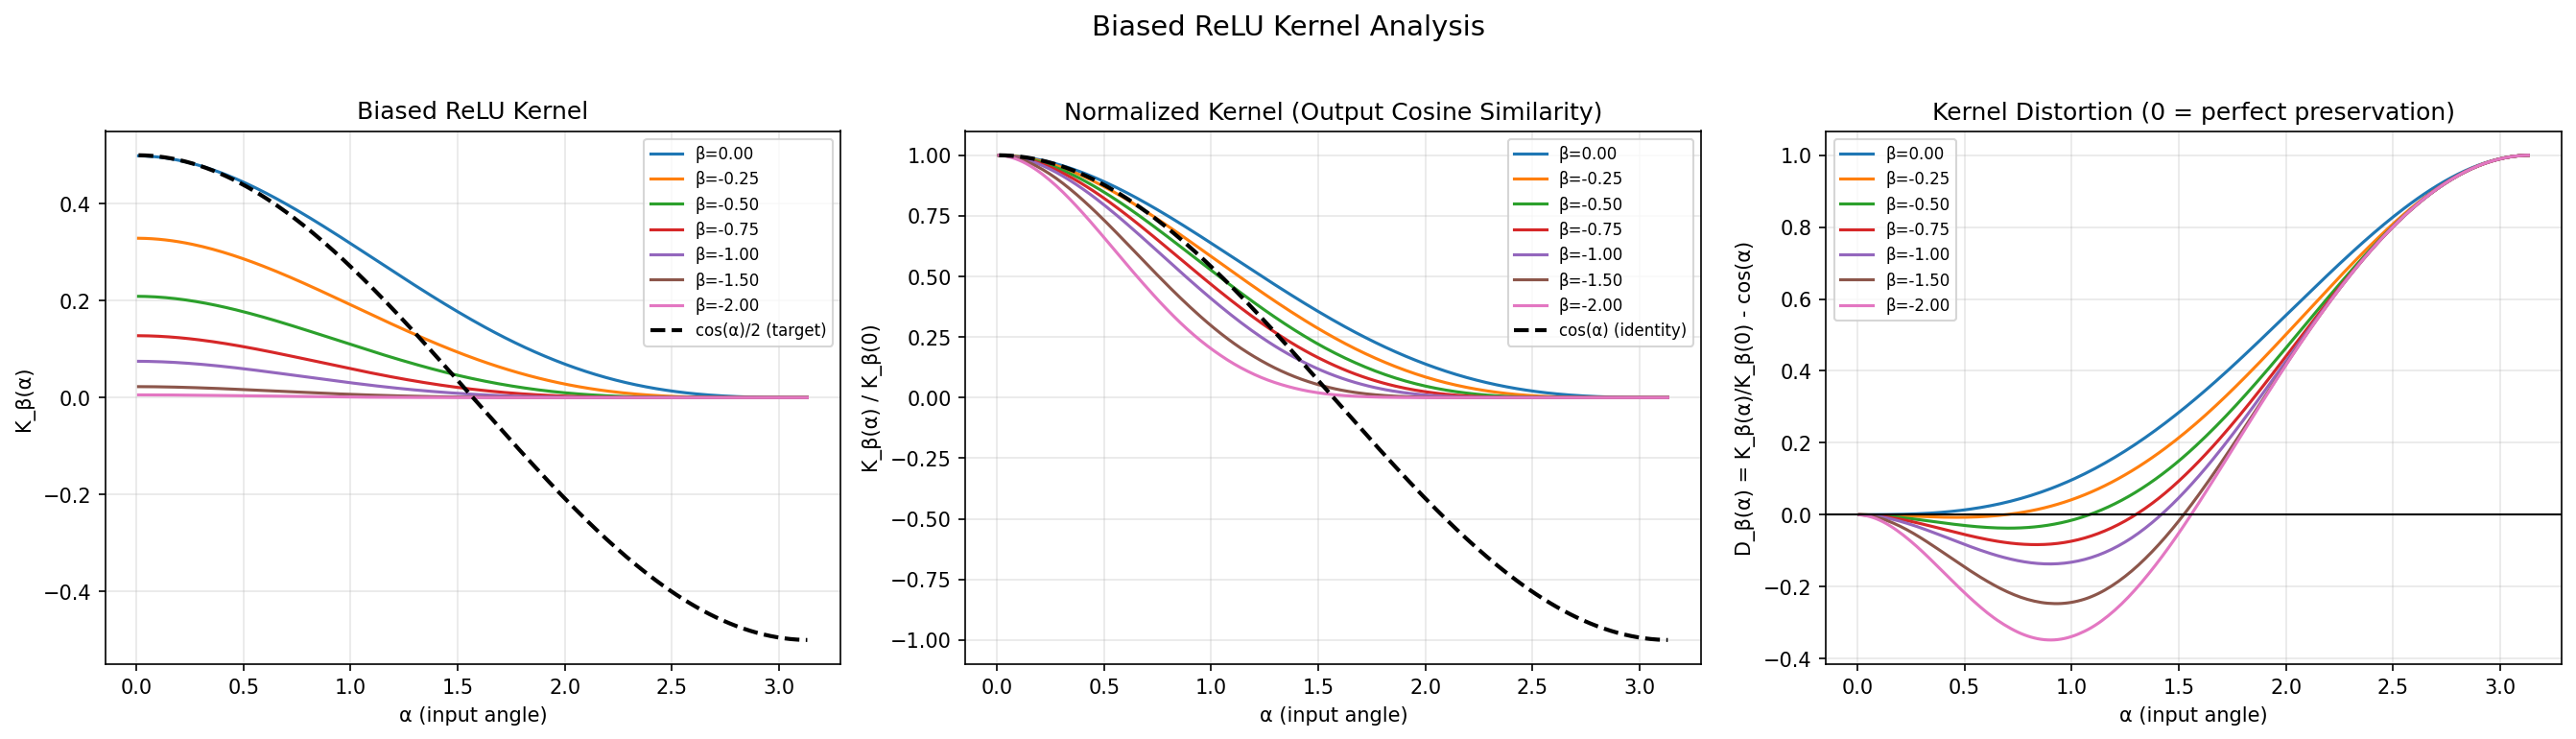
\includegraphics[width=\textwidth]{figures/biased_relu_kernel.png}
\caption{Biased ReLU kernel analysis.
  \textbf{Left:} Raw kernel $K_\beta(\alpha)$ for various $\beta$.
  \textbf{Center:} Normalized kernel (output cosine similarity).
  \textbf{Right:} Kernel distortion $D_\beta(\alpha)$ --- negative bias
  reduces distortion at small angles but overcorrects at large angles.
  Source: \texttt{notebooks/07\_kernel\_geometry\_analysis.ipynb}, Cell~11.}
\label{fig:biased_kernel}
\end{figure}

\subsection{Results}

\begin{center}
\begin{tabular}{cccc}
\toprule
$\beta$ & Integrated distortion & Survival rate $\Phi(\beta)$ &
$\sigma^2_{\mathrm{adj}}$ factor \\
\midrule
$0.00$ & 0.912 & 50.0\% & 1.00 \\
$-0.50$ & 0.843 & 30.9\% & 1.62 \\
$\bm{-0.93}$ & \textbf{0.795} & \textbf{17.6\%} & \textbf{5.72} \\
$-1.50$ & 0.847 & 6.7\% & 14.9 \\
$-2.00$ & 0.905 & 2.3\% & 43.5 \\
\bottomrule
\end{tabular}
\end{center}

\textbf{Optimal bias:} $\beta^* \approx -0.93$.
\textbf{Distortion reduction:} $0.795 / 0.912 = 0.87$, i.e., only a
\textbf{13\% improvement}.

\subsection{Why it doesn't work}

The distortion profiles reveal the mechanism:
\begin{itemize}
  \item For \textbf{small angles} ($\alpha < 1$): negative bias reduces
        distortion (nearby vectors become less artificially similar).
  \item For \textbf{large angles} ($\alpha > 2$): negative bias
        \textbf{overcorrects} --- vectors that were nearly orthogonal
        appear negatively correlated in the output.
  \item No value of $\beta$ reduces distortion uniformly across all
        angles.
\end{itemize}

\subsection{Variance compensation}

At $\beta^* = -0.93$, only 17.6\% of neurons fire, so the output
signal is much weaker.  To maintain the same forward signal strength
as standard He:
\[
  \sigma^2_{\mathrm{adj}}
  = \frac{2/d}{2\,\Phi(\beta^*)} \cdot C(\beta^*)^{-1}
  \approx 5.72 \cdot \frac{2}{d},
\]
where $C(\beta^*)$ is a correction factor from the second moment of
the truncated Gaussian.

This $5.72\times$ variance increase would push the backward gain
well above~1, potentially creating its own gradient instability.

\subsection{Assessment}

Negative bias is a \textbf{dead end}:
\begin{enumerate}
  \item Marginal improvement (13\% distortion reduction) ---
        insufficient to prevent collapse over 20+ layers.
  \item Extreme sparsity (82\% of neurons silent) requiring massive
        variance compensation.
  \item The distortion is reshaped, not eliminated.
  \item \textbf{Fundamental limit:} No pointwise nonlinearity
        (applied independently per neuron) can fully preserve the input
        kernel.  The distortion $D(\alpha)$ is intrinsic to any
        nonlinear map from $\R^2 \to \R$, and a threshold shift can
        only change $D$'s shape, not make it zero everywhere.
\end{enumerate}

% ──────────────────────────────────────────────────────────────────
\section{Analyzing Kernel-Preserving Optimizer Solutions}
\label{sec:kp_analysis}

\subsection{Motivation}

The \texttt{kernel\_preserving} initializer
(Section~\ref{sec:kp_init}) directly minimizes the kernel distortion.
At 5 layers it achieves $k$-NN $= 0.737$ (comparable to He).
By analyzing the structure of the optimized weight matrices, we ask:
\begin{itemize}
  \item Does the optimizer discover row centering?
  \item Does it discover negative bias?
  \item Or something entirely different?
\end{itemize}

We initialize 10 independent layers with \texttt{kernel\_preserving}
and compare the resulting weight matrices to standard He.

\subsection{Results}

\begin{table}[h]
\centering
\begin{tabular}{lccc}
\toprule
Property & He & KP & KP/He ratio \\
\midrule
Mean $|\text{row sum}|$ & 1.2 & 12.2 & $10\times$ \\
Mean row norm $\|\bm{w}_i\|$ & 1.3 & 15.0 & $11.5\times$ \\
Weight distribution & Gaussian & Uniform (flat) & --- \\
Mean pre-activation (DC) & 0.03 & 0.39 & $13\times$ \\
SVD spectrum & Flat ($\sim\!2.5$) & Decaying ($41 \to 20$) & --- \\
\bottomrule
\end{tabular}
\caption{Structural comparison of He vs.\ kernel-preserving weight matrices.}
\label{tab:kp_structure}
\end{table}

\begin{flagbox}
The inner-product and norm terms in the KP objective
\eqref{eq:kp_objective} are normalized by $d_{\mathrm{out}}$.
The norm constraint targets
$\|\relu(W\bm{x})\|^2 / d_{\mathrm{out}} \approx 1$,
which means $\|\relu(W\bm{x})\| \approx \sqrt{d_{\mathrm{out}}}$.
This targeting of output norms $\sqrt{d}$ rather than~$1$ contributes
to the observed $11.5\times$ weight inflation: part of the inflation
is an artifact of this normalization choice.
\end{flagbox}

\subsection{Key findings}

\begin{enumerate}
  \item \textbf{NOT row centering.}
        Row sums are $10\times$ \emph{larger} than He.
        The optimizer moves \textbf{away} from zero row sums.
        If centering were optimal for kernel preservation, the optimizer
        would have converged toward $\sum_j W_{ij} \approx 0$.

  \item \textbf{NOT negative bias.}
        The DC component (mean pre-activation) is $13\times$ larger than He.
        The optimizer \emph{amplifies} the mean, opposite to the biased
        ReLU strategy of Section~\ref{sec:biased_relu}.

  \item \textbf{Uniform, not Gaussian.}
        The weight elements follow a nearly uniform distribution (flat
        histogram, heavy-tailed Q-Q plot vs.\ normal), a radical departure
        from any standard initialization.

  \item \textbf{Anisotropic SVD.}
        The singular value spectrum decays from $\sim\!41$ (top) to
        $\sim\!20$ (bottom), with condition number $\sim\!2\times$
        (vs.\ $\sim\!1.1\times$ for He).
        The optimizer selectively amplifies certain input directions:
        components along top singular vectors get large pre-activations
        and survive ReLU with high probability, while components along
        bottom singular vectors are more likely killed.

  \item \textbf{Massively inflated weights.}
        Row norms $11.5\times$ larger than He.
        This inflation compounds catastrophically at depth:
        $15^L$ grows to astronomical values, causing the float64
        overflow at 20 layers (Section~\ref{sec:kp_failure}).
\end{enumerate}

\subsection{Why the structure is non-composable}

The KP optimizer's anisotropic amplification is tuned to the
\emph{input distribution} (random unit vectors).  After one KP layer
transforms the data, the output distribution is no longer unit vectors
--- it has been selectively amplified and truncated by ReLU.
The next layer's KP optimization, still targeting random unit vectors,
operates under violated assumptions.

Over $L$ layers, the accumulated mismatch between the assumed input
distribution (unit vectors) and the actual input distribution
(increasingly distorted post-ReLU data) causes the optimization to
diverge.

\subsection{Implications}

The optimizer confirms that kernel preservation requires a radically
different weight structure from any standard initialization.
The structure it finds (massive inflation + anisotropy + uniform
weights) is inherently per-layer and data-dependent --- there is no
simple closed-form generalization.

This reinforces the conclusion from Section~\ref{sec:biased_relu}:
the ReLU kernel distortion is a fundamental property of the nonlinearity
that cannot be eliminated by a single-layer weight structure,
regardless of its complexity.

% ══════════════════════════════════════════════════════════════════
\chapter{Two Collapse Modes: The Empirical Angle Map}
\label{ch:angle_map}
% ══════════════════════════════════════════════════════════════════

\noindent
This chapter provides the most intuitive visualization of why row
centering fails at geometry despite appearing to succeed in PCA plots.

% ──────────────────────────────────────────────────────────────────
\section{Single-Layer Angle Map: All Initializers Are Identical}
\label{sec:single_layer_map}

\subsection{Method}

We generate pairs of random unit vectors at controlled angles
$\alpha \in \{5^\circ, 10^\circ, \dots, 175^\circ\}$ in
$\R^{784}$, pass each pair through one initialized layer followed by
ReLU, and measure the output angle $\alpha'$ between the resulting
vectors.  We average over 200 pairs per angle and 5 random seeds.

\subsection{Results}

\begin{center}
\begin{tabular}{lcc}
\toprule
Initializer & Mean ratio $\alpha'/\alpha$ & Min ratio \\
\midrule
\texttt{he}                          & 0.7751 & 0.5081 \\
\texttt{orthogonal\_he}              & 0.7754 & 0.5081 \\
\texttt{row\_centered\_he\_var\_adj} & 0.7751 & 0.5081 \\
\texttt{kernel\_preserving}          & 0.7772 & 0.5081 \\
\bottomrule
\end{tabular}
\end{center}

All four initializers produce \textbf{identical} single-layer angle
maps (to within measurement noise).  The He empirical result matches
the theoretical prediction from the arc-cosine kernel
(equation~\eqref{eq:angle_map}) to within $0.14^\circ$.

\begin{figure}[h]
\centering
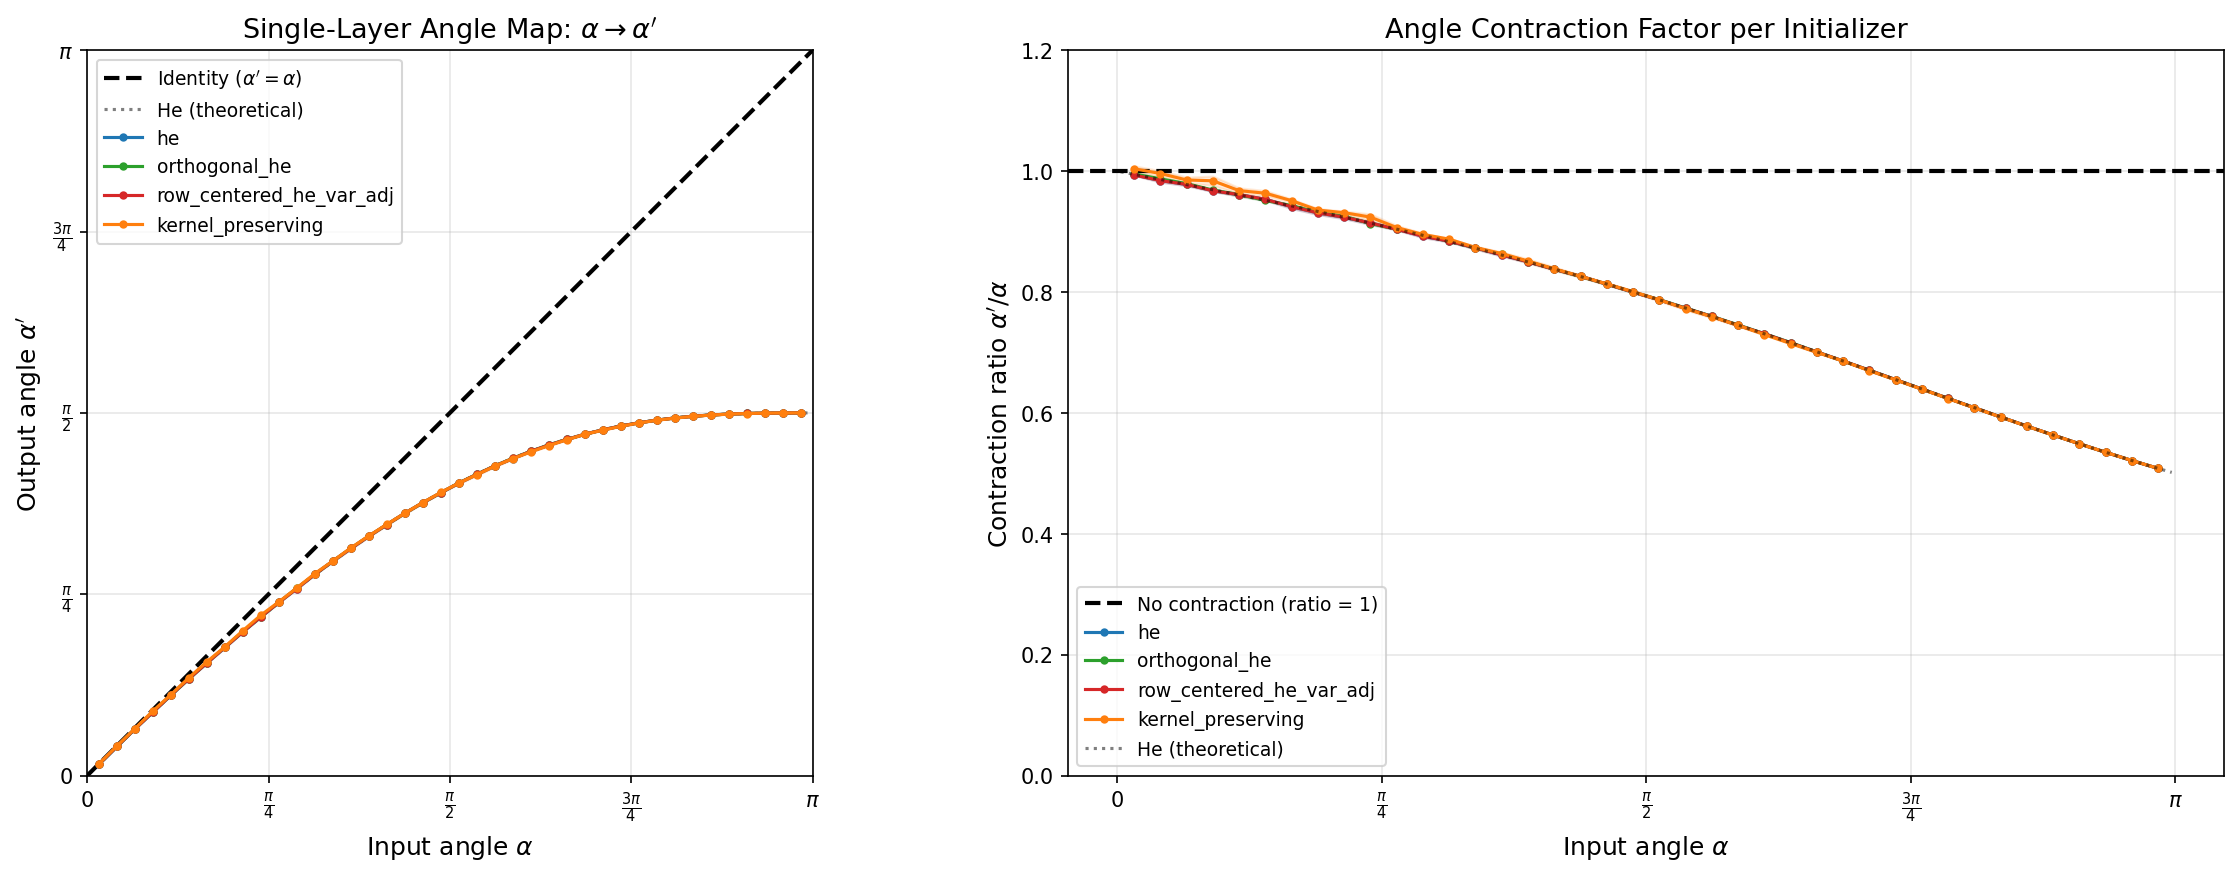
\includegraphics[width=\textwidth]{figures/single_layer_angle_map.png}
\caption{\textbf{Left:} Single-layer angle map $\alpha \to \alpha'$ for
  four initializers (empirical, 200 pairs $\times$ 5 seeds) vs.\ the
  theoretical arc-cosine kernel prediction.
  All initializers lie on top of the theory curve.
  \textbf{Right:} Contraction ratio $\alpha'/\alpha < 1$ for all angles.
  Source: \texttt{notebooks/07\_kernel\_geometry\_analysis.ipynb}, Cell~25.}
\label{fig:single_layer_angle_map}
\end{figure}

\subsection{Why row centering is invisible at one layer}

The experiment uses random \textbf{unit vectors} as inputs.
Unit vectors in high dimensions have near-zero mean:
$\bar{x} = (1/d)\sum_j x_j \approx 0$.  Therefore the DC component
is negligible, and the row centering constraint
$\sum_j W_{ij} = 0$ has almost no effect on the pre-activations
$z_i = \sum_j W_{ij} x_j \approx \sum_j W_{ij}(x_j - \bar{x})$.

\begin{proposition}
For unit vector inputs with zero DC component, the single-layer
angle contraction is determined entirely by the ReLU nonlinearity
(through the arc-cosine kernel $K(\alpha)$), independent of the
weight structure.
\end{proposition}

The differences between initializers emerge only from layer~2 onward,
when the inputs are \emph{post-ReLU activations} with a significant
positive DC component ($\E[a] = \sigma/\sqrt{2\pi} > 0$).

% ──────────────────────────────────────────────────────────────────
\section{Multi-Layer Angle Evolution: Two Different Fixed Points}
\label{sec:two_fixed_points}

\subsection{Method}

Track the angle between a pair of vectors as they propagate through
$L = 20$ layers.  Start from four initial angles:
$\alpha_0 \in \{30^\circ, 60^\circ, 90^\circ, 120^\circ\}$.
Average over 200 pairs and 5 seeds.

\subsection{Results}

\begin{table}[h]
\centering
\begin{tabular}{lcccc}
\toprule
Initializer & $30^\circ \to 20\text{L}$ &
$60^\circ \to 20\text{L}$ &
$90^\circ \to 20\text{L}$ &
$120^\circ \to 20\text{L}$ \\
\midrule
\texttt{he}           & $13.8^\circ$ & $17.4^\circ$ & $18.6^\circ$ & $19.0^\circ$ \\
\texttt{orthogonal\_he} & $12.5^\circ$ & $15.6^\circ$ & $16.8^\circ$ & $17.3^\circ$ \\
\texttt{rc\_var\_adj} & $\bm{70.9^\circ}$ & $\bm{71.3^\circ}$ & $\bm{71.3^\circ}$ & $\bm{71.7^\circ}$ \\
\bottomrule
\end{tabular}
\caption{Output angles after 20 layers.  He converges toward $0^\circ$;
row-centered converges to ${\sim}71^\circ$.}
\label{tab:angle_evolution}
\end{table}

\textbf{He / orthogonal:}
All starting angles contract toward $\bm{0^\circ}$ --- classical
geometric collapse where all representations align
(\emph{identity collapse}).

\textbf{Row-centered:}
All starting angles converge to $\bm{\sim\!71^\circ}$ --- every pair
of points becomes equidistant (\emph{equidistance collapse}).

% ──────────────────────────────────────────────────────────────────
\section{Why $71^\circ$ Is the Row-Centered Fixed Point}
\label{sec:why_71}

\subsection{The mechanism}

\begin{enumerate}
  \item Row centering strips the DC component from post-ReLU
        activations at each layer
        (Proposition~\ref{prop:dc_blind}).
  \item The remaining AC component (directional information) decays
        by $0.826\times$ per layer (equation~\eqref{eq:rc_fwd_gain}).
  \item After enough layers, only random fluctuations from the weight
        matrices remain.
  \item The activations at each layer are non-negative (post-ReLU).
        Random non-negative vectors in high dimension have pairwise
        angles concentrated around a characteristic value determined by
        the geometry of the positive orthant.
\end{enumerate}

\subsection{The positive orthant angle}

For random non-negative vectors $\bm{a}, \bm{b} \in \R_{\geq 0}^d$
with i.i.d.\ entries drawn from a half-Gaussian, the expected cosine
similarity concentrates (for large~$d$) around:
\begin{equation}
  \E\!\left[\frac{\langle \bm{a}, \bm{b} \rangle}
    {\|\bm{a}\| \cdot \|\bm{b}\|}\right]
  \approx \frac{(\E[a_j])^2}{\E[a_j^2]}
  = \frac{1/(2\pi)}{1/2}
  = \frac{1}{\pi}
  \approx 0.318,
\end{equation}
where we used the half-Gaussian moments
(Lemma~\ref{lem:half_gaussian}) with $\sigma^2 = 1$:
$\E[a_j] = 1/\sqrt{2\pi}$, so $(\E[a_j])^2 = 1/(2\pi)$, and
$\E[a_j^2] = 1/2$.
This gives the expected angle:
\begin{equation}\label{eq:fixed_point}
  \alpha^*
  = \arccos\!\left(\frac{1}{\pi}\right)
  \approx 71.5^\circ.
\end{equation}

\begin{remark}
The predicted fixed point ($71.5^\circ$) matches the empirically
observed value ($\sim\!71^\circ$) to within measurement noise.
This excellent agreement confirms the mechanism: after enough layers
of DC stripping and signal decay, the post-ReLU activations become
effectively random non-negative vectors, and their pairwise angles
concentrate at $\arccos(1/\pi)$ --- a universal constant determined
solely by the geometry of the positive orthant and the half-Gaussian
distribution.
\end{remark}

% ──────────────────────────────────────────────────────────────────
\section{Connecting to the $k$-NN Results}
\label{sec:connecting_knn}

The two fixed points provide the most intuitive explanation of the
geometry results from Chapter~\ref{ch:geometry}:

\begin{center}
\begin{tabular}{lll}
\toprule
Property & He (fixed point $0^\circ$) & RC (fixed point $71^\circ$) \\
\midrule
Failure mode & All vectors align & All vectors become equidistant \\
What survives & Relative ordering & Spread (dimensionality) \\
$k$-NN at 20\,L & 0.639 (degrades slowly) & 0.110 (chance) \\
$d_{\mathrm{eff}}$ at 20\,L & 5.8 (collapsed) & 388 (high) \\
\bottomrule
\end{tabular}
\end{center}

Both are geometric collapse, but they destroy \textbf{different}
aspects of the input geometry:

\begin{itemize}
  \item \textbf{He} preserves \textbf{ordering} (which vectors are
        closer to each other) but loses \textbf{scale} (all angles
        shrink toward~$0^\circ$).  Since $k$-NN classification depends
        only on the ranking of distances, not their absolute values,
        He maintains usable class structure.

  \item \textbf{Row-centered} preserves \textbf{scale} (angles stay
        around $71^\circ$, not shrunk to zero) but loses
        \textbf{ordering} (all pairwise angles become identical,
        so there is no way to tell which points were originally
        in the same class).
\end{itemize}

For classification tasks, \textbf{ordering is more important than
scale} --- explaining why He ($k$-NN $= 0.639$) vastly outperforms
row-centered ($k$-NN $= 0.110$) despite having lower effective
dimensionality.

% ══════════════════════════════════════════════════════════════════
\chapter{Conclusions and Open Questions}
\label{ch:conclusions}
% ══════════════════════════════════════════════════════════════════

% ──────────────────────────────────────────────────────────────────
\section{Summary of Proven Results}

\begin{enumerate}
  \item \textbf{The gradient trap is structural}
        (Chapter~\ref{ch:gradient_trap}).
        Row centering creates a forward gain of
        $\sqrt{(\pi-1)/\pi} \approx 0.826$ per layer, with a locked
        forward/backward ratio of $0.827$.  This was confirmed
        empirically (single-sample experiments reproduce the same
        pattern; variance sweep shows constant ratio across all
        variance factors).  No scalar variance adjustment can make
        both gains equal to~1 simultaneously.

  \item \textbf{Row centering destroys class structure at depth}
        (Chapter~\ref{ch:geometry}).
        Using $k$-NN accuracy as the geometry metric,
        \texttt{row\_centered\_he\_var\_adj} drops to chance level
        (0.110) by 20 layers.  Standard He stays at 0.639.
        The PCA scatter plots that previously suggested geometry
        preservation were measuring \emph{spread}, not
        \emph{structure}.

  \item \textbf{Forward decay kills both geometry and gradients}
        (Chapters~\ref{ch:gradient_trap}--\ref{ch:geometry}).
        These are the same phenomenon: the $0.826^L$ signal decay
        randomizes activations at depth (destroying class
        information) and creates non-uniform gradients (preventing
        learning).

  \item \textbf{Partial centering and layer-balanced are partial fixes}
        (Chapter~\ref{ch:fixing_trap}).
        The alpha sweep reveals a Pareto frontier with no escape.
        The layer-balanced approach ($\eta = 0.5$) reduces gradient
        ratio from $11\times$ to $4\times$ while keeping full geometry,
        but the backward gain of 1.21 limits further improvement.

  \item \textbf{Negative bias cannot fix the kernel}
        (Section~\ref{sec:biased_relu}).
        Optimal $\beta^* \approx -0.93$ reduces distortion by only 13\%,
        at the cost of 82\% silent neurons and $5.7\times$ variance
        compensation.  No pointwise nonlinearity can fully preserve
        the input kernel.

  \item \textbf{The kernel-preserving optimizer confirms centering is
        wrong} (Section~\ref{sec:kp_analysis}).
        The optimizer discovers the \emph{opposite} of row centering
        (large row sums, inflated weights, anisotropic structure), but
        this solution is non-composable across layers.

  \item \textbf{Two different collapse modes}
        (Chapter~\ref{ch:angle_map}).
        He collapses to $0^\circ$ (identity: all vectors align).
        Row-centered collapses to $71^\circ$ (equidistance: all
        vectors become equidistant).
        Both destroy class information, but He preserves
        \emph{ordering} (which $k$-NN needs) while row-centered
        destroys it.

  \item \textbf{Orthogonal\_he is the practical winner}
        (Section~\ref{sec:orthogonal_analysis}).
        It achieves $k$-NN $= 0.662$ at 20 layers (vs.\ He's 0.639),
        a $\sim\!3.6\%$ improvement from reduced variance, with no
        gradient trap.
\end{enumerate}

% ──────────────────────────────────────────────────────────────────
\section{The Real Enemy: $D(\alpha) > 0$}

The systematic ReLU kernel distortion
\[
  D(\alpha) = \frac{1}{\pi}\bigl(\sin\alpha - \alpha\cos\alpha\bigr) > 0
  \quad\text{for all } \alpha \in (0,\pi)
\]
affects \textbf{all} initializers.  No single-layer weight structure
can eliminate it:
\begin{itemize}
  \item The distortion depends on the normalized kernel
        $\hat{K}(\alpha) = K(\alpha)/K(0)$, which is invariant to
        weight scaling.
  \item Orthogonal matrices have the same marginal distribution as
        Gaussian, so the same $\hat{K}$.
  \item Row centering changes the effective kernel but introduces worse
        problems (forward decay, equidistance collapse).
  \item Negative bias reshapes $D_\beta(\alpha)$ but cannot make it
        zero everywhere.
  \item The kernel-preserving optimizer finds a complex solution that
        works per-layer but is non-composable.
\end{itemize}

This distortion is \textbf{fundamental to any pointwise nonlinearity}:
the operation
$\E[\phi(\bm{w}^\top \bm{x}_i) \cdot \phi(\bm{w}^\top \bm{x}_j)]$
cannot equal $\langle \bm{x}_i, \bm{x}_j \rangle$ for all angles
unless $\phi$ is linear.

% ──────────────────────────────────────────────────────────────────
\section{Open Questions}

\begin{enumerate}
  \item \textbf{Reframing row centering in the thesis.}
        The advisor proposed row centering specifically for geometry
        preservation.  Our results show it is worse than standard He
        for class separability.  How should we present this finding
        diplomatically while being scientifically rigorous?

  \item \textbf{Pivoting toward bounding the distortion.}
        If the kernel distortion cannot be eliminated, perhaps the
        thesis contribution is proving this impossibility and
        characterizing the best achievable bounds.  What is the
        optimal single-layer angle map achievable by any weight
        structure?

  \item \textbf{Multi-layer or joint optimization.}
        The kernel-preserving optimizer fails because each layer is
        optimized independently.  Could jointly optimizing all layers
        (accounting for cumulative kernel drift) produce a composable
        solution?

  \item \textbf{Alternative activation functions.}
        The distortion $D(\alpha) > 0$ is specific to ReLU.
        Activation functions with $\E[\phi(z)] = 0$ (e.g., centered
        ReLU, GELU minus its mean, or antisymmetric activations) would
        eliminate the DC problem that drives the row-centering failure.
        Do they also reduce the kernel distortion?

  \item \textbf{Practical implications.}
        For networks trained with gradient descent (not just random
        projections), does the initialization-time geometry matter?
        The gradient trap prevents early learning, but adaptive
        optimizers (Adam, LARS) may compensate.
\end{enumerate}


\bibliographystyle{plain}
\bibliography{references}

\end{document}
